\documentclass{book}

\usepackage{fontspec} % used to import Calibri
\usepackage{anyfontsize} % used to adjust font size

% needed for inch and other length measurements
% to be recognized
\usepackage{calc}

% for colors and text effects as is hopefully obvious
\usepackage[dvipsnames]{xcolor}
\usepackage{soul}

% control over margins
\usepackage[margin=1in]{geometry}
\usepackage[strict]{changepage}

\usepackage{mathtools}
\usepackage{amsfonts}
\usepackage{bm}

\usepackage[scr=rsfso, scrscaled=.96]{mathalpha}

\usepackage{amssymb} % originally imported to get the proof square
\usepackage{xfrac}
\usepackage[overcommands]{overarrows} % Get my preferred vector arrows...
\usepackage{relsize}

% Just am using this to get a dashed line in a table...
% Also you apparently want this to be inactive if you aren't
% using it because it slows compilation.
\usepackage{arydshln} \ADLinactivate 
\newenvironment{allowTableDashes}{\ADLactivate}{\ADLinactivate}

\usepackage{graphicx}
\graphicspath{{./158_Images/}}

\usepackage{tikz}
   \usetikzlibrary{arrows.meta}
   \usetikzlibrary{graphs, graphs.standard}

\usepackage{quiver} %commutative diagrams


\newfontfamily{\calibri}{Calibri}
\setlength{\parindent}{0pt}
\definecolor{RawerSienna}{HTML}{945D27}

% ~~~~~~~~~~~~~~~~~~~~~~~~~~~~~~~~~~~~~~~~~~~~~~~~~~
%Arrow Commands:

% Thank you Bernard, gernot, and Sigur who I copied this from:
% https://tex.stackexchange.com/questions/364096/command-for-longhookrightarrow
\newcommand{\hooklongrightarrow}{\lhook\joinrel\longrightarrow}
\newcommand{\hooklongleftarrow}{\longleftarrow\joinrel\rhook}
\newcommand{\hookxlongrightarrow}[2][]{\lhook\joinrel\xrightarrow[#1]{#2}}
\newcommand{\hookxlongleftarrow}[2][]{\xleftarrow[#1]{#2}\joinrel\rhook}

% Thank you egreg who I copied from:
% https://tex.stackexchange.com/questions/260554/two-headed-version-of-xrightarrow
\newcommand{\longrightarrowdbl}{\longrightarrow\mathrel{\mkern-14mu}\rightarrow}
\newcommand{\longleftarrowdbl}{\leftarrow\mathrel{\mkern-14mu}\longleftarrow}

\newcommand{\xrightarrowdbl}[2][]{%
  \xrightarrow[#1]{#2}\mathrel{\mkern-14mu}\rightarrow
}
\newcommand{\xleftarrowdbl}[2][]{%
  \leftarrow\mathrel{\mkern-14mu}\xleftarrow[#1]{#2}
}

\newcommand{\MRoman}[1]{%
   \textrm{\MakeUppercase{\romannumeral #1}}%
}

% ~~~~~~~~~~~~~~~~~~~~~~~~~~~~~~~~~~~~~~~~~~~~~~~~~~

\newcommand{\learnToSpot}[1]{{\color{Red}#1}}

\newcommand{\hOne}{%
   \color{Black}%
   \fontsize{14}{16}\selectfont%
}
\newcommand{\hTwo}{%
\color{MidnightBlue}%
   \fontsize{13}{15}\selectfont%
}
\newcommand{\hThree}{%
   \color{PineGreen!85!Orange}
   \fontsize{12}{14}\selectfont%
}
\newcommand{\hFour}{%
   \color{Cyan}
   \fontsize{12}{14}\selectfont%
}
\newcommand{\myComment}{%
   \color{RawerSienna}%
   \fontsize{12}{14}\selectfont%
}
\newcommand{\teachComment}{
   \color{Orange}%
   \fontsize{12}{14}\selectfont%
}
\newcommand{\exOne}{%
   \color{Purple}%
   \fontsize{13}{15}\selectfont%
}
\newcommand{\exTwo}{%
   \color{Purple}%
   \fontsize{13}{15}\selectfont%
}
\newcommand{\exP}{%
   \color{Purple}%
   \fontsize{12}{14}\selectfont%
}
\newcommand{\exTwoP}{%
   \color{RedViolet}%
   \fontsize{13}{15}\selectfont%
}
\newcommand{\exPP}{%
   \color{RedViolet}%
   \fontsize{12}{14}\selectfont%
}
\newcommand{\exPPP}{%
   \color{VioletRed}%
   \fontsize{12}{14}\selectfont%
}
% ~~~~~~~~~~~~~~~~~~~~~~~~~~~~~~~~~~~~~~~~~~~~~~~~

\newcommand{\cyPen}[1]{{\vphantom{.}\color{Cerulean}#1}}
\newcommand{\redPen}[1]{{\vphantom{.}\color{Red}#1}}

\newenvironment{myIndent}{%
   \begin{adjustwidth}{2.5em}{0em}%
}{%
   \end{adjustwidth}%
}

\newenvironment{myDindent}{%
   \begin{adjustwidth}{5em}{0em}%
}{%
   \end{adjustwidth}%
}

\newenvironment{myTindent}{%
   \begin{adjustwidth}{7.5em}{0em}%
}{%
   \end{adjustwidth}%
}

\newenvironment{myConstrict}{%
   \begin{adjustwidth}{2.5em}{2.5em}%
}{%
   \end{adjustwidth}%
}

\newcommand{\udefine}[1]{{%
   \setulcolor{Red}%
   \setul{0.14em}{0.07em}%
   \ul{#1}%
}}

\newcommand{\blab}[1]{\textbf{#1}}

\newcommand{\uuline}[2][.]{%
{\vphantom{a}\color{#1}%
\rlap{\rule[-0.18em]{\widthof{#2}}{0.06em}}%
\rlap{\rule[-0.32em]{\widthof{#2}}{0.06em}}}%
#2}

\newcommand{\pprime}{{\prime\prime}}
\newcommand{\suchthat}{ \hspace{0.3em}s.t.\hspace{0.3em}}
\newcommand{\rea}[1]{\mathrm{Re}(#1)}
\newcommand{\ima}[1]{\mathrm{Im}(#1)}
\newcommand{\comp}{\mathsf{C}}
\newcommand{\card}{\mathrm{card}}
\newcommand{\diam}{\mathrm{diam}}
\newcommand{\myHS}{ \hspace{0.5em}}

\newcommand{\myId}{\mathrm{Id}}
\newcommand{\myIm}{\mathrm{im}}
\newcommand{\myObj}{\mathrm{Obj}}
\newcommand{\myHom}{\mathrm{Hom}}
\newcommand{\myEnd}{\mathrm{End}}
\newcommand{\myAut}{\mathrm{Aut}}

\newcommand{\brm}[1]{\bm{\mathrm{#1}}}

\newcommand{\qbinom}{\genfrac{[}{]}{0pt}{}}

\newcommand{\mcateg}[1]{{\bm{\mathsf{#1}}}}

\newcommand{\mdeg}{\mathrm{mdeg}\phantom{.}}

% Thank you Gonzalo Medina and Moriambar who wrote this on stack exchange:
%https://tex.stackexchange.com/questions/74125/how-do-i-put-text-over-symbols%
\newcommand{\myequiv}[1]{\stackrel{\mathclap{\mbox{\footnotesize{$#1$}}}}{\equiv}}

% Thank you chs who wrote this on stack exchange:
%https://tex.stackexchange.com/questions/89821/how-to-draw-a-solid-colored-circle%
\newcommand{\filledcirc}[1][.]{\ensuremath{\hspace{0.05em}{\color{#1}\bullet}\mathllap{\circ}\hspace{0.05em}}}

%Thank you blerbl who wrote this on stack exchange:
%https://tex.stackexchange.com/questions/25348/latex-symbol-for-does-not-divide
\newcommand{\ndiv}{\hspace{-0.3em}\not|\hspace{0.35em}}

\newcommand{\mySepOne}[1][.]{%
   {\noindent\color{#1}{\rule{6.5in}{1mm}}}\\%
}
\newcommand{\mySepTwo}[1][.]{%
   {\noindent\color{#1}{\rule{6.5in}{0.5mm}}}\\%
}

\newenvironment{myClosureOne}[2][.]{%
   \color{#1}%
   \begin{tabular}{|p{#2in}|} \hline \\%
}{%
   \\ \hline \end{tabular}%
}

\newcommand{\retTwo}{\hfill\bigbreak}

\newcommand{\mHeader}[1]{{
   \color{Black}%
   \fontsize{20}{18}\selectfont%
   #1\retTwo
}}


\title{Math 188 Notes (Professor: Steven Sam)}
\author{Isabelle Mills}

\begin{document}
\maketitle{}
\setul{0.14em}{0.07em}
\calibri

\hOne
\mHeader{Lecture 1 Notes: 9/27/2024}

\blab{Linear Recurrence Relations:}\\
A sequence $(a_n)_{n \geq 0}$ satisfies a \udefine{linear recurrence relation of order $d$} if there exists\\ $c_1, \ldots, c_d$ with $c_d \neq 0$ so that $a_n = c_1a_{n-1} + c_2a_{n-2} + \ldots + c_da_{n-d}$ for all $n \geq d$.

\begin{myTindent}\myComment
   (For $0 \leq n < d$, we usually explicitely specify $a_n$. Also, it seems like we are\\ assuming all $a_n$ and $c_n$ are complex numbers right now)\retTwo
\end{myTindent}

To start this course, we're gonna discuss finding explicit (non-recursive) solutions.\retTwo

Firstly, if $d = 1$, then this problem is easy. We can just plug in previous elements repeatedly to get that:

{\centering $a_n = c_1a_{n-1} = c_1^{\vphantom{|}2}a_{n-2} = \ldots = c_1^{\vphantom{|}n}a_0$ \retTwo\par}

If $d = 2$, then plugging in previous elements doesn't help us really anymore. So how do we solve this problem now?\\

\begin{myIndent}\hTwo
   \blab{Theorem:} Consider the \udefine{characteristic polynomial} $t^2 - c_1t - c_2$ and let $r_1, r_2$\\ be the roots of that polynomial. If $r_1 \neq r_2$, then there exists $\alpha_1, \alpha_2$ such that\\ $a_n = \alpha_1r_1^{\vphantom{|}n} + \alpha_2r_2^{\vphantom{|}n}$ for all $n \geq 0$.\retTwo

   To solve for $\alpha_1$ and $\alpha_2$, plug in different values of $n$ into our equation. Since $r_1 \neq r_2$, we know the below linear system has a unique solution:

   {\centering $ 
   \begin{matrix}
      a_0 = \alpha_1 + \alpha_2 \\ a_1 = \alpha_1 r_1 + \alpha_2 r_2
   \end{matrix}$ \retTwo\par}
\end{myIndent}

Now backing up, why does the above method work?\\
\begin{myIndent}\hTwo

   \blab{Approach 1: (Vector Spaces)}\\
   The set of sequences $(a_n)_{n\geq 0}$ form a vector space. Furthermore given any constants $c_1$ and $c_2$, we know that the set of sequences satisfying $a_n = c_1a_{n-1} + c_2a_{n-2}$ for all $n \geq 2$ is a subspace.
   
   \begin{myIndent}\hThree
      Proof:\\
      Suppose $(a_n)$ and $(b_n)$ both satisfy that $a_n = c_1a_{n-1} + c_2a_{n-2}$ and\\ $b_n = c_1b_{n-1} + c_2b_{n-2}$. Then given any constants $\gamma$ and $\delta$, we have that:

      {\centering $(\gamma a_n + \delta b_n) = c_1(\gamma a_{n-1} + \delta b_{n-1}) + c_2(\gamma a_{n-2} + \delta b_{n-2})$ \retTwo\par}

      Hence, all linear combinations of any two sequences satisfying our linear\\ recurrence relation also satisfies our linear recurrence relation.\retTwo
   \end{myIndent}

   Now what our above theorem is stating is that the sequences $(r_1^{\vphantom{|}n})$ and $(r_2^{\vphantom{|}n})$ span the subspace of solutions to our linear recurrence relation.\retTwo

   To see this, first note that $(r_1^{\vphantom{|}n})$ and $(r_2^{\vphantom{|}n})$ satisfy our recurrence relation.
   \begin{myIndent}\hThree
      If $n \geq 2$, then $r_i^{\vphantom{|}n} - c_1r_i^{\vphantom{|}n-1} - c_2r_i^{\vphantom{|}n-2} = r_i^{\vphantom{|}n-2}(r_i^{\vphantom{|}2} - c_1r_i - c_2) = r_i^{\vphantom{|}n-2} (0)$.\\ Hence, we know that $r_i^{\vphantom{|}n} = c_1r_i^{\vphantom{|}n-1} + c_2r_i^{\vphantom{|}n-2}$ for all $n \geq 2$.\newpage
   \end{myIndent}

   Also, since we assumed $r_1 \neq r_2$, we know that $(r_1^{\vphantom{|}n})$ is linearly independent to $(r_2^{\vphantom{|}n})$. And finally, as mentioned before, we can solve a linear system of equations to find\\ [-2pt] coffecients for a linear combination of $(r_1^{\vphantom{|}n})$ and $(r_2^{\vphantom{|}n})$ equal to any other sequence satisfying our recurrence relation.\retTwo

   \blab{Approach 2: (Formal Power Series)}\\
   Define the power series $A(x) = \sum\limits_{n \geq 0}a_nx^n$. We call $A(x)$ a \udefine{generating function} of\\ [-10pt] the sequence $(a_n)$.
   
   
   \begin{myTindent}\begin{myIndent}\teachComment
      (We'll treat the formal power series more rigorously later...)\retTwo
   \end{myIndent}\end{myTindent}

   Now note that:\\ [-10pt]
   \begin{myIndent}\hThree
      \begin{tabular}{l}
         $ A(x) = a_0 + a_1x + \sum\limits_{n \geq 2} a_nx^n$\\ [14pt]
         $ \phantom{A(x)} = a_0 + a_1x + \sum\limits_{n \geq 2} (c_1a_{n-1} + c_2a_{n-2})x^n$\\ [14pt]
         $ \phantom{A(x)} = a_0 + a_1x + c_1\sum\limits_{n \geq 2} a_{n-1}x^n + c_2\sum\limits_{n \geq 2}a_{n-2}x^n$\\ [14pt]
         $\phantom{A(x)} = a_0 + a_1x + c_1(A(x) - a_0)x + c_2(A(x))x^2$
      \end{tabular}\retTwo
   \end{myIndent}

   Isolating $A(x)$, we get the equation: $A(x) = \dfrac{a_0 + a_1x - a_0c_1x}{1 - c_1x - c_2x^2}$.\retTwo

   Next, let's do fraction decomposition on our equation for $A(x)$.
   \begin{myIndent}\hThree
      \blab{Issue:} We defined $r_1$ and $r_2$ as the roots of $t^2 - c_1t - c_2 = (t - r_1)(t - r_2)$.\retTwo

      \blab{Trick:} Plug in $t = \frac{1}{x}$. That way, we have that:
      
      {\centering$x^{-2} - c_1x^{-1} - c_2 = (x^{-1} - r_1)(x^{-1} - r_2)$.\retTwo\par}
      
      After that, multiply both sides of our equation by $x^2$ to get that:

      {\centering $ 1 - c_1x - c_2x^2 = (1 - r_1x)(1 - r_2x)$ \retTwo\par}
   \end{myIndent}

   Since we're assuming $r_1 \neq r_2$, we know that for some constants $\alpha_1$ and $\alpha_2$, we have that:

   {\centering $A(x) = \dfrac{\alpha_1}{1 - r_1x} + \dfrac{\alpha_2}{1 - r_2x} $ \retTwo\par}

   
   \begin{myTindent}\begin{myIndent}\teachComment
      (If $r_1 = r_2$, then this step is where things will go differently.)\retTwo
   \end{myIndent}\end{myTindent}

   Now finally, we can rewrite $\frac{\alpha_1}{1 - r_1x}$ as the geometric series $\alpha_1 \sum\limits_{n \geq 0}(r_1x)^n$. Doing\\ [-6pt] likewise with $\frac{\alpha_2}{1 - r_2x}$, we get that:

   {\center $A(x) = \sum\limits_{n \geq 0} a_n x^n = \alpha_1 \sum\limits_{n \geq 0}(r_1x)^n + \alpha_2 \sum\limits_{n \geq 0}(r_2x)^n = \sum\limits_{n \geq 0}(\alpha_1r_1^{\vphantom{|}n} + \alpha_2r_2^{\vphantom{|}n})x^n$ \retTwo\par}

   Hence, we have for each $n$ that $a_n = \alpha_1r_1^{\vphantom{|}n} + \alpha_2r_2^{\vphantom{|}n}$.
\end{myIndent}

\newpage

\mHeader{Lecture 2: 9/30/2024}

\begin{myIndent}\hTwo
   \blab{Approach 3: (Matrices)}\\
   If $a_n = c_1a_{n-1} + c_2a_{n-2}$, then we can say that: $\begin{bmatrix}c_1 & c_2 \\ 1 & 0\end{bmatrix}\begin{bmatrix}a_{n-1} \\ a_{n-2}\end{bmatrix} = \begin{bmatrix}a_n \\ a_{n-1}\end{bmatrix}$\retTwo

   Letting $\bm{C} = 
   \begin{bmatrix}
      c_1 & c_2 \\ 1 & 0
   \end{bmatrix}$, we thus know that: $\bm{C}^n \begin{bmatrix}a_1 \\ a_0\end{bmatrix} = \begin{bmatrix}a_{n+1} \\ a_{n}\end{bmatrix}$\retTwo

   Notably, the characteristic polynomial of $\bm{C}$ is $t^2 - c_1t - c_2$. So the eigenvalues of $\bm{C}$ are $r_1$ and $r_2$. Because we assumed $r_1$ and $r_2$ are distinct, we know $\bm{C}$  is\\ diagonalizable. Hence there exists an invertible matrix $\bm{B}$ such that:
   
   {\center$\bm{B}
   \begin{bmatrix}
      r_1 & 0 \\ 0 & r_2
   \end{bmatrix}\bm{B}^{-1} = \bm{C}$\retTwo\par}

   Now set $\begin{bmatrix} x \\ y\end{bmatrix} = \bm{B}^{-1}\begin{bmatrix} a_1 \\ a_0\end{bmatrix}$. Then we can see that:

   {\center $\begin{bmatrix}
      a_{n+1} \\ a_n
   \end{bmatrix} =
   \bm{C}^n\begin{bmatrix}
      a_1 \\ a_0
   \end{bmatrix} = \bm{B}\bm{D}^n\begin{bmatrix}
      x \\ y
   \end{bmatrix} = \bm{B}\begin{bmatrix}
      r_1^{\vphantom{|}n}x \\ r_2^{\vphantom{|}n}y
   \end{bmatrix} = \begin{bmatrix}
     b_{1,1} r_1^{\vphantom{|}n}x + b_{1,2}r_2^{\vphantom{|}n}y \\ b_{2,1} r_1^{\vphantom{|}n}x + b_{2,2}r_2^{\vphantom{|}n}y
   \end{bmatrix}$ \retTwo\par}

   Setting $\alpha_1 = b_{2,1}x$ and $\alpha_2 = b_{2,2}y$, we have thus found constants $\alpha_1$ and $\alpha_2$ such that $a_n = \alpha_1r_1^{\vphantom{|}n} + \alpha_2r_2^{\vphantom{|}n}$.\retTwo\retTwo
\end{myIndent}

\hOne
Now some further questions to ask about recurrence relations are:
\begin{enumerate}
   \item What if $r_1 = r_2$?
   \item What if $d \geq 3$?
   \item What if the recurrence relation is non-homogeneous or non-linear?\retTwo
\end{enumerate}

To start, let's answer question 1.
\begin{myIndent}\hTwo
   \blab{Theorem:} Suppose $r_1$ and $r_2$ are the roots of $t^2 - c_1t - c_2$ with $r_1 = r_2$. Then there exists $\alpha_1, \alpha_2$ such that $a_n = \alpha_1r_1^{\vphantom{|}n} + \alpha_2 n r_1^{\vphantom{|}n}$ for all $n \geq 0$.\retTwo

   As was true when $r_1 \neq r_2$, you can solve for $\alpha_1$ and $\alpha_2$ by plugging in different values of $n$ into the equation in order to get a linear system of equations.\retTwo
\end{myIndent}

To explain why this is, let's revisit two of our previous approaches.\retTwo

\begin{myIndent}\hTwo
   \blab{The Formal Power Series Approach Revisited:}\\
   Before, we were able to show that $A(x) = \dfrac{a_0 + (a_1 - a_0c_1)x}{(1 - r_1x)(1 - r_2x)}$ without assuming\\ [-7pt] anything about $r_1$ and $r_2$.\newpage

   But when we assume $r_1 = r_2$, we then get a different partial fraction decomposition for $A(x)$. Specifically, we have that there exists constants $\beta_1, \beta_2$ such that:

   {\centering $A(x) = \dfrac{\beta_1}{1 - r_1x} + \dfrac{\beta_2}{(1 - r_1x)^2} $ \retTwo\par}

   Now we'll go into more rigor later. But for now, note that:

   {\centering $\frac{1}{(1 - y)^2} = \left(\frac{1}{1 - y}\right)^\prime = \left(\sum\limits_{n\geq 0}y^n\right)^\prime = \sum\limits_{n \geq 1}ny^{n-1} = \sum\limits_{n \geq 0}(n+1)y^n$\par}

   
   \begin{myTindent}\myComment
      Comment from the future: as we'll cover two lectures from now, the definition of a derivative of a formal power series is different from the analysis definition we're familiar with.\retTwo
   \end{myTindent}

   Hence, we can write $A(x) = \sum\limits_{n \geq 0}a_n x^n = (\beta_1 + \beta_2) \sum\limits_{n \geq 0}r_1^{\vphantom{|}n}x^n + \beta_2 \sum\limits_{n \geq 0}nr_1^{\vphantom{|}n}x^n$.\retTwo

   Or in other words, setting $\alpha_1 = \beta_1 + \beta_2$ and $\alpha_2 = \beta_2$, we have that:

   {\centering $a_n = \alpha_1r_1^{\vphantom{|}n} + \alpha_2 n r_1^{\vphantom{|}n}$\\ [20pt]\par}

   \blab{The Matrix Approach Revisited:}\\

   If $r_1 = r_2$, then we must hav ethat the matrix $\bm{C}$ is not diagonalizable. For suppose it was, meaning there exists an invertible matrix $\bm{B}$ such that:
   
   {\centering$\bm{C} = \bm{B}
   \begin{bmatrix}
      r_1 & 0\\ 0 & r_1
   \end{bmatrix}\bm{B}^{-1}$\retTwo\par}

   Then we'd have to have that $\bm{C} = r_1\bm{B}\bm{B}^{-1} = 
   \begin{bmatrix}
      r_1 & 0 \\ 0 & r_1
   \end{bmatrix}$. But we know $\bm{C}$ isn't that.\retTwo

   Since we know $\bm{C}$ Is not diagonalizable, we will instead use the \textit{Jordan-normal form} of $\bm{C}$. Specifically, we know there exists an invertible matrix $\bm{B}$ such that:

   {\centering $\bm{C} = \bm{B}
   \begin{bmatrix}
      r_1 & 1 \\ 0 & r_1
   \end{bmatrix}\bm{B}^{-1}$\par}
   
   \begin{myDindent}\begin{myDindent}\myComment
      Don't worry for the time being about how to prove the Jordan-normal form of a matrix always exists.\retTwo
   \end{myDindent}\end{myDindent}

   This tells us that $\bm{C}^n = 
   \bm{B}\begin{bmatrix}
      r_1 & 1 \\ 0 & r_1
   \end{bmatrix}^n\bm{B}^{-1}$.\retTwo Also, you can show by induction that $\begin{bmatrix}
      r_1 & 1 \\ 0 & r_1
   \end{bmatrix}^n = \begin{bmatrix}
      r_1^n & nr_1^{n-1} \\ 0 & r_1^n
   \end{bmatrix}$.

   So finally, defining $
   \begin{bmatrix}
      x \\ y
   \end{bmatrix}$ as before and expanding out the expression, you can get\\ [-8pt] \phantom{aaaaaaaaaaaaaaaaaaaaaaaaaaaaaaaaaaaaaaaaaaaaaaa} an explicit equation for $a_n$.\newpage
\end{myIndent}

As for answering question 2, if $d \geq 3$, then our characteristic polynomial becomes $t^d - c_1t^{d-1} - \ldots - c_d$. We'll assume this polynomial has distinct roots $r_1, \ldots, r_m$ with multiplicities $s_1, \ldots, s_m$ respectively.\retTwo


\begin{myIndent}\hTwo
   \blab{Theorem:} There exists constants $\alpha_1, \ldots, \alpha_d$ such that:

   {\center $a_n = \sum\limits_{i = 1}^{s_1} \alpha_i n^{\vphantom{|}i-1} r_1^{\vphantom{|}n} + \ldots + \hspace{-2em}\sum\limits_{i = s_1 + \ldots + s_{m-1} + 1}^{s_1 + \ldots + s_m}\hspace{-2em} \alpha_i n^{\vphantom{|}i-1}r_m^{\vphantom{|}n}$ \retTwo\par}

   As before, to solve for $\alpha_1$ through $\alpha_d$, you can plug in values of $n$ and solve a linear system of equations.\retTwo

   \begin{myIndent}\hThree
      The approaches to prove this are the same as when $d = 2$. However, there are just more terms floating around that need to be dealt with.\retTwo
   \end{myIndent}
\end{myIndent}

Special case: suppose the characteristic polynomial is $(t - 1)^d$.

\begin{myIndent}\hTwo
   In that case, because the root of the polynomial $r$ is $1$, there exists $\alpha_1, \ldots, \alpha_d$\\ such that 
   
   {\centering $a_n = \alpha_1 + n\alpha_2 + n^2\alpha_3 + \ldots + n^{d-1}\alpha_d$. \retTwo\par}
   
   In other words, the formula for $a_n$ is a polynomial in $n$.\retTwo
\end{myIndent}

\mySepTwo

\blab{Another perspective on the characteristic polynomial}:\\

Let $V$ be the vector space of sequences $(a_n)_{n\geq 0}$, and define the \udefine{translation operator} $T: V \longrightarrow V$ such that $(a_n)_{n \geq 0} \mapsto (a_{n+1})_{n\geq 0}$. Now, given $\bm{a} \in V$ and the recurrence relation $a_n = c_1a_{n-1} + \ldots + c_da_{n-d}$ for all $n \geq d$, we have that $\bm{a}$ satisfies our recurrence relation if and only if:

{\centering $T^d\bm{a} = c_1T^{d-1}\bm{a} + c_2T^{d-2}\bm{a} + \ldots + c_d\bm{A}$ \retTwo\par}

In other words, we must have that $\bm{a} \in \ker(T^d - c_1T^{d-1} - \ldots - c_d)$.\retTwo

If $r_1, \ldots, r_d$ are the roots of the characteristic polynomial $t^d - c_1T^{d-1} - \ldots - c_d$, then we can rewrite this as:

{\centering $(T - r_1)\cdots(T - r_d)\bm{a} = \bm{0}$ \retTwo\par}

\begin{myIndent}\hTwo
   \blab{Proposition:} Given a sequence $\bm{a} = (a_n)_{n \geq 0}$, there exists a polynomial $p(n)$ of\\ degree at most $d - 1$ such that $a_n = p(n)$ if and only if $(T - 1)^d\bm{a} = \bm{0}$.

   \begin{myIndent}\hThree
      We already saw in the special case above one direction of this statement. As for the other direction, suppose $p(n) = \alpha_d n^{d-1} + \alpha_{d-1}n^{d-2} + \ldots + \alpha_1$. Then $(T - 1)$ applied to the sequence $(p(n))_{n\geq 0}$ is the sequence $(p(n + 1) - p(n))_{n \geq 0}$ Importantly, $p(n + 1)$ is also a polynomial of degree $d - 1$ with $\alpha_d$ as the coefficient in front of $n^{d - 1}$. So the difference is a polynomial of degree at most $d - 2$.\newpage

      Proceeding by induction, we know that $(T - 1)^d(p(n))_{n\geq 0} = \bm{0}$.\retTwo
   \end{myIndent}   
\end{myIndent}

Note that the operator $(T - 1)$ can be thought of as the taking the "derivative" of a sequence $\bm{a}$. Going by that analogy, the previous proposition is saying that a sequence $\bm{a}$ is given by a polynomial if and only if a derivative of some order of the sequence is zero. Interestingly, the same is true of differential equations.\retTwo

\mySepTwo

\mHeader{Lecture 3: 10/2/2024}

To quickly address question 3, in general there is no unified approach to dealing with nonlinear recurrence relations. However, we can often solve non-homogeneous\\ linear recurrence relations.
\begin{myIndent}\exOne
   This will be addressed by the homework (see HW 1: Exercise (2)).\retTwo
\end{myIndent}

\blab{Formal Power Series:}

A \udefine{formal power series} in the variable $x$ is an expression of the form $A(x) = \sum\limits_{n \geq 0} a_n x^n$\\ [-8pt] where $a_n$ is a sequence of elements of a field.

\begin{myTindent}\teachComment
   Technically, we can go more general to a commutative ring (but we won't).\retTwo
\end{myTindent}

We call $A(x)$ the \udefine{generating function} of $(a_n)_{n \geq 0}$.\retTwo

If $A(x)$ and $B(x)$ are the generating functions of $(a_n)_{n \geq 0}$ and $(b_n)_{n \geq 0}$ respectively, then:
\begin{itemize}
   \item $A(x) = B(x)$ iff $a_n = b_n$ for all $n$.
   \item $A(x) + B(x) \coloneq \sum\limits_{n \geq 0}(a_n + b_n)x^n$.\\ [-16pt]
   \item $A(x)B(x) \coloneq \sum\limits_{n \geq 0}c_nx^n$ where $c_n = \sum\limits_{i = 0}^n a_ib_{n-i}$.\\ [-12pt]
    
    \begin{myTindent}\myComment
      (in other words this is the Cauchy Product of $A(x)$ and $B(x)$)\retTwo
    \end{myTindent}
\end{itemize}

Note that polynomials and constants are special cases of formal power series with the sequence generating that function being eventually zero.\retTwo

Also, sums and products of formal power series satisfy the commutative, associative, and distributive properties of a field.

\begin{myIndent}\myComment
   The only one of those properties that's non-trivial to show is the associativity of products. One way that you can prove this property is to show that :

   {\center $\sum\limits_{i = 0}^n \sum\limits_{j = 0}^i a_jb_{i-j}c_{n-i} = \hspace{-0.8em}\sum\limits_{(p, q, r) \in I}\hspace{-0.8em}a_p b_q c_r = \sum\limits_{i = 0}^n \sum\limits_{j = 0}^i a_{n-i}b_{j}c_{i - j}$,\par}

   where $I = \{(p, q, r) \in \mathbb{Z}^3 \mid p + q + r = n \text{ and } p, q, r \geq 0\}$.\newpage
\end{myIndent}

Plus, letting $0 + 0x + \ldots$\phantom{a}  be the additive identity, then given any formal power series $A(x) = \sum\limits_{n \geq 0}a_n x^n$, we have that:

{\centering $-A(x) = (-1 + 0x + \ldots)\sum\limits_{n \geq 0}a_nx^n = \sum\limits_{n \geq 0}(-a_n)x^n$ is the additive inverse of $A(x)$.\retTwo\par}

Finally, we clearly have that $1 + 0x + 0x^2 + \ldots$\phantom{a} is a multiplicative identity of the set of formal power series.\retTwo

Therefore, to make this perfectly clear, the set of formal power series is not actually a set of functions. Rather, given a field (or commutative ring) $F$, the set of formal power series with coefficients in that ring is a commutative ring on the set $F^{\omega}$ of infinite sequences of elements of $F$ using the $+$ and $\cdot$ operations defined above.

\begin{myIndent}\myComment
   In other words, it doesn't make sense to plug values of $x$ into formal power series. Rather, the power series notation is just to make it clearer where the definitions of different\\ operations are coming from.\retTwo

   Also, since the set of formal power series on a commutative ring is itself a commutative ring, you can define the set of formal power series on the set of formal power series on that commutative ring. Spoiler: this is a way to define multivariate formal power series.\retTwo
\end{myIndent}

\mySepTwo

A formal power series $A(x)$ is \udefine{invertible} if there exists a formal power series $B(x)$ such that $A(x)B(x) = 1$. We write $B(x) = A(x)^{-1} = \frac{1}{A(x)}$, and call $B(x)$ the\\ [-2pt] \udefine{inverse} of $A(x)$.\retTwo

\begin{myIndent}\hTwo
   \blab{Example:} If $A(x) = \sum\limits_{n \geq 0} x^n$, then $A(x)$ is invertible with inverse $B(x) = 1 - x$.

   \begin{myIndent}\hThree
      Proof:\\ [-10pt]

      \begin{tabular}{l}
         $A(x)B(x) = (1 + x +x^2 + \ldots)(1 - x)$ \\ $\phantom{A(x)B(x)} = 1 + x - x + x^2 - x^2 + x^3 - x^3 + \ldots = 1$
      \end{tabular}\\

      So $\sum\limits_{n \geq 0} x^n = \frac{1}{1 - x}$.\retTwo
   \end{myIndent}

   \blab{Theorem:} $A(x) = \sum\limits_{n \geq 0}a_n$ is invertible if and only if $a_0$ has a multiplicative inverse.
   
   \begin{myIndent}\hThree
      Proof:\\
      If there exists $B(x)$ such that $A(x)B(x) = 1$, then we must have that:
      \begin{myIndent}
         \begin{tabular}{l}
            $a_0 b_0 = 1$ \\
            $a_0 b_1 + a_1 b_0 = 0$ \\
            $a_0 b_2 + a_1 b_1 + a_2 b_0 = 0$ \\
            $\phantom{a_0b_2 + a_1b_1 +} \vdots $
         \end{tabular}\newpage
      \end{myIndent}

      If $\frac{1}{a_0}$ exists then we can inductively solve for each $b_n$. Specifically, $b_0 = \frac{1}{a_0}$ and\\ [-3pt] $b_n = -\frac{1}{a_0}\sum\limits_{i=1}^n a_i b_{n - i}$. Then $B(x) = \sum\limits_{n \geq 0}b_n x^n$ satisfies that $A(x)B(x) = 1$.\retTwo

      If $\frac{1}{a_0}$ doesn't exist, then there is no choice of $b_0$ such that $A(x) (\sum\limits_{n \geq 0}b_n x^n) = 1$.\\ [-6pt] So $A(x)$ has no inverse.\retTwo
   \end{myIndent}
\end{myIndent}

\mHeader{Lecture 4: 10/4/2024}

If $A(x)$ is a power series and $n \geq 0$, then $[x^n]A(x)$ refers to the coefficient $a_n$ in front of $x^n$.\retTwo

Let $A_0(x), A_1(x), \ldots$ be a sequence of formal power series. We say the sequence \udefine{formally converges} to $A(x)$ if:

{\centering $\forall n \geq 0, \exists N \geq 0 \suchthat i \geq N \Longrightarrow [x^n]A_i(x) = [x^n]A(x)$ \retTwo\par}

We also write this as $\lim\limits_{i \rightarrow \infty}A_i(x) = A(x)$

\begin{myTindent}\teachComment
   Note that this definition is different from the familiar definition of\\ convergence in 140. For instance, the sequence $A_i(x) = \frac{1}{i + 1}$ doesn't\\ formally converge.\retTwo
\end{myTindent}

\begin{myIndent}\hTwo
   \blab{Lemma:} Suppose $\lim\limits_{i \rightarrow \infty} A_i(x) = A(x)$ and $\lim\limits_{i \rightarrow \infty} B_i(x) = B(x)$. Then:
   \begin{itemize}
      \item $\lim\limits_{i \rightarrow \infty} (A_i(x) + B_i(x)) = A(x) + B(x)$
      \item $\lim\limits_{i \rightarrow \infty} (A_i(x)B_i(x)) = A(x)B(x)$
   \end{itemize}
   \begin{myIndent}\hThree
      The proof for this is rather trivial. So do it yourself. :P\retTwo
   \end{myIndent}
\end{myIndent}

Continuing to let $A_0(x), A_1(x), \ldots$, be a sequence of formal power series, we define:

\begin{myIndent}
   $\sum\limits_{i \geq 0} A_i(x) \coloneq \lim\limits_{i \rightarrow \infty} (\sum\limits_{j = 0}^i A_j(x))$\\

   $\prod\limits_{i \geq 0} A_i(x) \coloneq \lim\limits_{i \rightarrow \infty}(\prod\limits_{j = 0}^i A_j(x))$\retTwo

   \hTwo\blab{Lemma:} {\hThree (This is just reapplying the previous lemma for sequences and using the\\ \phantom{aaaaaaaaaaaaaaaaaaaaaaaaaaaaaaaaaaaaaaaaaaaaaaaaa} commutative property\dots)}
   \begin{itemize}
      \item If $\sum\limits_{i \geq 0}A_i(x)$ and $\sum\limits_{i \geq 0}B_i(x)$ exist, then:
      
      {\centering $\sum\limits_{i \geq 0}(A_i(x) + B_i(x)) = \sum\limits_{i \geq 0}A_i(x) + \sum\limits_{i \geq 0}B_i(x)$.\retTwo\par}
   
      \item If $\prod\limits_{i \geq 0}A_i(x)$ and $\prod\limits_{i \geq 0}B_i(x)$ exist, then:\\ [-13pt]
      
      {\centering$\prod\limits_{i \geq 0}(A_i(x)B_i(x)) = \left(\prod\limits_{i \geq 0}A_i(x)\right)\hspace{-0.4em}\left(\prod\limits_{i \geq 0}B_i(x)\right)$.\newpage\par}
   \end{itemize}
\end{myIndent}

Given a formal power series $A(x)$, we define:

{\centering $\mdeg A(x) \coloneq \inf(\{n \in \mathbb{Z}_+ \cup \{0\} \mid [x^n]A(x) \neq 0\} \cup \{\infty\})$.\retTwo\par}

\begin{myIndent}\hTwo
   \blab{Proposition:} Suppose $A_0(x), A_1(x), \ldots$ is a sequence of formal power series.
   \begin{itemize}
      \item $\sum\limits_{i \geq 0} A_i(x)$ exists if and only if $\lim\limits_{i \rightarrow \infty} \mdeg A_i(x) = \infty$.
      
      \begin{myIndent}\hThree
         Proof: {\myComment(The professor skipped this because he thinks it's boring.)}

         ($\Longleftarrow$)\\ [2pt]
         Suppose $\lim\limits_{j \rightarrow \infty} \mdeg A_j(x) = \infty$. Then for all $n \geq 0$, there exists $N \geq 0$ such that $\mdeg A_j(x) > n$ for all $j > N$. So:
         
         {\centering $[x^n]\left(\sum\limits_{j = 0}^i A_j(x)\right) = [x^n]\left(\sum\limits_{j = 0}^N A_j(x)\right)$ for all $i > N$.\retTwo\par}

         ($\Longrightarrow$)\\ [2pt]
         Suppose that $\lim\limits_{j \rightarrow \infty} \mdeg A_j(x)$ either doesn't exist or doesn't equal infinity if\\ [-1pt] it does exist. Then we know there must exist $N$ such that $\mdeg A_j(x) < N$\\ [3pt] for infinitely many $j \geq 0$. In turn, for some $n \in \{0, 1, \ldots, N - 1\}$, there\\ [3pt] must be infinitely many $j \geq 0$ such that $\mdeg A_j(x) = n$. Thus, there does\\ [3pt] not exist $M \geq 0$ such that:

         {\centering $[x^n]\left(\sum\limits_{j = 0}^i A_j(x)\right)$ is the same for all $i \geq M$.  \retTwo\par}
      \end{myIndent}
      
      \item Assume each $A_i$ has no constant term. Then $\prod\limits_{i \geq 0}(1 + A_i(x))$ exists if and only\\ [-8pt] if $\lim\limits_{i \rightarrow \infty} \mdeg A_i(x) = \infty$.
      
      \begin{myIndent}\hThree
         Proof: {\myComment (btw I'm having to figure this all out without any outside help)}\\
         \blab{Lemma:} Suppose $B(x)$ and $C(x)$ are formal power series such that\\ $[x^0]B(x) = 1$ and $\mdeg C(x) = n$. Then $\mdeg B(x)C(x) = n$ with\\ $[x^n](B(x)C(x)) = [x^n](C(x))$.\retTwo

         \blab{Corollary 1:} Given $B(x)$ and $C(x)$ defined as before, for all $0 \leq i < n$:
         
         {\centering $[x^i](B(x)(1 + C(x))) = [x^i](B(x) + B(x)C(x)) = [x^i](B(x))$.\retTwo\par}

         \blab{Corollary 2:} $[x^0]\left(\prod\limits_{j = 0}^i (1 + A_j)\right) = 1$ for all $i \geq 0$.\retTwo

         ($\Longleftarrow$)\\
         Suppose $\lim\limits_{j \rightarrow \infty} \mdeg A_j(x) = \infty$. Then for any $n \geq 0$, there exists $N \geq 0$\\ [-1pt] such that $\mdeg A_j(x) > n$ for all $j > N$. So given any $i > N$, we can\\ [3pt] inductively show using the above lemma and corollaries that:\newpage

         {\centering 
         \begin{tabular}{l}
            $[x^n]\left(\prod\limits_{j = 0}^{i}(1 + A_j(x))\right) = [x^n]\left(\prod\limits_{j = 0}^{i - 1}(1 + A_j(x))\right)$ \\ $\phantom{aaaaaaaaaaaaaaaaaa} = \cdots = [x^n]\left(\prod\limits_{j = 0}^N(1 + A_j(x))\right)$
         \end{tabular} \retTwo\par}

         ($\Longrightarrow$)\\
         As before, we can show there must be infinitely many $i \geq 0$ such that\\ $\mdeg A_i(x) = n$ for some $n$. And for any such $i$, we have by the above\\ lemma that:

         {\centering 
         \begin{tabular}{l}
            $[x^n]\left(\prod\limits_{j = 0}^i (1 + A_j(x))\right)$ \\ $\phantom{aaaaa} = [x^n]\left(\prod\limits_{j = 0}^{i -1}(1 + A_j(x)) + \left(\prod\limits_{j = 0}^{i -1}(1 + A_j(x))\right)A_i(x)\right)$ \\ [8pt]
            $\phantom{aaaaaaaaaa} = [x^n]\left(\prod\limits_{j = 0}^{i -1}(1 + A_j(x))\right) + [x^n]A_i(x) $\\ [8pt]
            $\phantom{aaaaaaaaaaaaaaa} \neq [x^n]\left(\prod\limits_{j = 0}^{i -1}(1 + A_j(x))\right)$
         \end{tabular}\retTwo\par}

         So there is no $N \geq 0$ such that:

         {\centering $[x^n]\left(\prod\limits_{j = 0}^i(1 + A_j(x))\right)$ is the same for all $i \geq N$.  \retTwo\par}
      \end{myIndent}
   \end{itemize}
\end{myIndent}

\mySepTwo

Suppose $A(x)$ and $B(x)$ are formal power series such that $A(x)$ has no constant term and $B(x) = \sum\limits_{n \geq 0}b_n x^n$. Then we define their \udefine{composition}: \\ [-12pt]

{\centering $\phantom{aaaaaaa}(B \circ A)(x) = B(A(x)) \coloneq \sum\limits_{n \geq 0}b_n A(x)^n$ \retTwo\par}

\begin{myIndent}\hTwo
   This is well defined because $\mdeg A(x) \geq 1 \Longrightarrow \mdeg A(x)^n \geq n$. Therefore,\\ $\lim\limits_{n \rightarrow \infty} b_n A(x)^n = \infty$, meaning we can apply the previous proposition.\retTwo

   Special Case: If $A(x) = 0$, then $(B \circ A)(x) = b_0$.\retTwo

   \exOne\blab{Proposition:} If $A(x)$, $B(x)$, and $C(x)$ are power series generated by $(a_n)_{n \geq 0}$, $(b_n)_{n \geq 0}$, and $(c_n)_{n \geq 0}$ respectively such that $(B \circ A)(x)$ and $(C \circ A)(x)$ are defined, then:
   
   \begin{itemize}
      \item $((B + C) \circ A)(x) = (B \circ A)(x) + (C \circ A)(x)$
      
      \begin{myIndent}\exTwoP
         Proof:\\
         By the second lemma on page 9, we know that:\\\exPP
         $\sum\limits_{n \geq 0}(b_n + c_n)A(x)^n  = \sum\limits_{n \geq 0}(b_n A(x)^n + c_n A(x)^n) = \sum\limits_{n \geq 0}b_n A(x)^n + \sum\limits_{n \geq 0}c_n A(x)^n$
         \retTwo
      \end{myIndent}

      \item $((BC) \circ A)(x) = (B \circ A)(x)(C \circ A)(x)$\newpage
      
      \begin{myIndent}\exTwoP
         Proof:\\
         By the first lemma on page 9, we know that:

         {\centering\exPP 
         \begin{tabular}{l}
            $(B \circ A)(x)(C \circ A(x)) = \left(\lim\limits_{n \rightarrow \infty}\left(\sum\limits_{i = 0}^n b_i A(x)^i\right)\right)\left(\lim\limits_{n \rightarrow \infty}\left(\sum\limits_{i = 0}^n c_i A(x)^i\right)\right)$\\ [10pt] $\phantom{(B \circ A)(x)(C \circ A(x))} = \lim\limits_{n \rightarrow \infty}\left(\left(\sum\limits_{i = 0}^n b_iA(x)^i\right)\left(\sum\limits_{i = 0}^n c_iA(x)^i\right)\right)$
         \end{tabular} \retTwo\par}

         Next note that given any $n \geq 0$, there exists a formal power series $R_n(x)$ with $\mdeg R_n(x) > n$ such that:
         
         {\centering$\left(\sum\limits_{i = 0}^n b_iA(x)^i\right)\hspace{-0.3em}\left(\sum\limits_{i = 0}^n c_iA(x)^i\right) = \sum\limits_{i = 0}^n \left(\sum\limits_{j = 0}^i b_jc_{i-j}\right)\hspace{-0.1em}A(x)^i + R_n(x)$\retTwo\par}

         Since $\lim\limits_{n \rightarrow \infty}\left(\sum\limits_{i = 0}^n \left(\sum\limits_{j = 0}^i b_jc_{i-j}\right)\hspace{-0.1em}A(x)^i\right) = ((BC) \circ A)(x)$ and\\ $\lim\limits_{n \rightarrow \infty}(R_n(x)) = 0$, we can thus apply the first lemma on page 9\\ [4pt] again to get that:

         {\centering\exPP 
         \begin{tabular}{l}
            $\lim\limits_{n \rightarrow \infty}\left(\left(\sum\limits_{i = 0}^n b_iA(x)^i\right)\left(\sum\limits_{i = 0}^n c_iA(x)^i\right)\right)$ \\ [12pt]
            $\phantom{aaaaaaaa} = \lim\limits_{n \rightarrow \infty}\left(\sum\limits_{i = 0}^n \left(\sum\limits_{j = 0}^i b_jc_{i-j}\right)\hspace{-0.1em}A(x)^i\right) + \lim\limits_{n \rightarrow \infty}(R_n(x))$\\ [16pt]
            $\phantom{aaaaaaaa} = ((BC) \circ A)(x) + 0$
         \end{tabular} \retTwo\par}
      \end{myIndent}
   \end{itemize}
\end{myIndent}

\mySepTwo

Suppose $A(x)$ is a formal power series. We define its \udefine{derivative}:

{\centering $(DA)(x) = A^\prime(x) \coloneq \sum\limits_{n \geq 1}n a_n x^{n - 1} = \sum\limits_{n \geq 0}(n + 1)a_{n + 1}x^n $\par}

\begin{myTindent}\teachComment
   Note that for $n \in \mathbb{Z}^+$ and $a_n \in F$, we define $n a_n$ via repeated addition.\retTwo
\end{myTindent}


\begin{myIndent}\hTwo
   \blab{Proposition:} The following rules hold for any two formal power series $A(x)$ and $B(x)$:
   \begin{itemize}
      \item Sum Rule: $(A + B)^\prime(x) = A^\prime(x) + B^\prime(x)$
      \begin{myIndent}\hThree
         This identity is hopefully obvious.\\ [-12pt]
      \end{myIndent}
      \item Product Rule: $(AB)^\prime(x) = A^\prime(x) B(x) + A(x) B^\prime(x)$
      \begin{myIndent}\hThree
         The proof for this identity requires rearranging sums strategically.\\ [-12pt]
      \end{myIndent}
      \item Power Rule: $(A^n)^\prime(x) = n A^{n-1}(x) A^\prime(x)$ if $n > 0$ and $(A^n)^\prime(x) = 0$ if $n = 0$.
      \begin{myIndent}\hThree
         To prove this, do induction on $n$ using the product rule.\newpage
      \end{myIndent}
   \end{itemize}
   
   Also if $[x^0]A(x) = 0$, then:
   \begin{itemize}
      \item Chain Rule: $(B \circ A)^\prime(x) = A^\prime(x) B^\prime(A(x))$
      
      \begin{myIndent}\hThree
         Proof: {\myComment(seriously I'm doing this proof on my own\dots I order you to give me pity.)}\\ [-6pt]

         \blab{Lemma:} If $A_0(x), A_1(x), \ldots$ are a sequence of formal power series that\\ converges to $A(x)$, then $\lim\limits_{n \rightarrow \infty} A_n^\prime(x) = A^\prime(x)$.

         \begin{myIndent}\hFour
            The proof for this is rather trivial. However, this is notably different from the convergence of derivatives of sequences of functions in math 140.\retTwo
         \end{myIndent}

         Now suppose $B(x) = \sum\limits_{n \geq 0}b_nx^n$, and for each $n$, set $B_n(x) = \sum\limits_{i = 0}^n b_i x^i$.\\ [2pt]
         By definition, we know that:\\ [-18pt]
         
         {\centering $\lim\limits_{n \rightarrow \infty}( (B_n \circ A)(x)) = \lim\limits_{n \rightarrow \infty}\left( \sum\limits_{i = 0}^n b_i A(x)^i\right) = (B \circ A)(x)$.\retTwo\par}

         Hence, applying the previous lemma, we know that:
         
         {\centering$\lim\limits_{n\rightarrow \infty}((B_n \circ A)^\prime(x)) = (B \circ A)^\prime(x)$.\retTwo\par}

         But now note that by the sum and power rules:

         {\centering
         \begin{tabular}{l}
            $(B_n \circ A)^\prime(x) = \sum\limits_{i = 0}^n b_i (A^i)^\prime(x)$\\ [4pt]
            $\phantom{(B_n \circ A)^\prime(x)} = \sum\limits_{i = 1}^{n}ib_i A(x)^{i-1}A^\prime(x) = A^\prime(x) \sum\limits_{i = 0}^{n-1}(i + 1)b_{i + 1} A(x)^i$\\ [4pt]
            $\phantom{(B_n \circ A)^\prime(x) = \sum\limits_{i = 1}^{n}ib_i A(x)^{i-1}A^\prime(x)} = A^\prime(x)(B_{n}^\prime \circ A)(x)$
         \end{tabular}\retTwo\par}

         Finally, by definition we know that:\\ [-16pt]

         {\centering $\lim\limits_{n \rightarrow \infty}( (B_{n}^\prime \circ A)(x)) = \lim\limits_{n \rightarrow \infty}\left( \sum\limits_{i = 0}^{n - 1} (i + 1) b_{i + 1} A(x)^i\right) = (B^\prime \circ A)(x)$.\retTwo\par}

         So by applying the first lemma on page 9, we know that:
         
         {\centering$\lim\limits_{n\rightarrow \infty}((B_n \circ A)^\prime(x)) = \lim\limits_{n\rightarrow \infty}(A^\prime(x)(B_{n}^\prime \circ A)(x)) = A^\prime(x)(B^\prime \circ A)(x)$\retTwo\par}
      \end{myIndent}
   \end{itemize}

   Meanwhile, if $A(x)$ is invertible, then:
   \begin{itemize}
      \item Multiplicative inverse rule: $(\frac{1}{A(x)})^\prime = \frac{-A^\prime(x)}{A(x)^2}$
      \begin{myIndent}\hThree
         To prove this, just apply product rule to the expression $A(x)(\frac{1}{A(x)}) = 1$.\retTwo
      \end{myIndent}
   \end{itemize}
\end{myIndent}

\exOne\mySepTwo

Examples of proving identities:\\ [-10pt]

\exPP
\begin{enumerate}
   \item Since $\frac{1}{1-x} = \sum\limits_{n \geq 0}x^n$, we know $-\frac{-1}{(1-x)^2} = (\frac{1}{1-x})^\prime = \left(\sum\limits_{n \geq 0}x^n\right)^\prime = \sum\limits_{n \geq 0}(n + 1)x^n$.
   \item $\sum\limits_{n \geq 0}nx^n = \sum\limits_{n \geq 0}(n + 1)x^n - \sum\limits_{n \geq 0}x^n = \frac{1}{(1-x)^2} - \frac{1}{1-x}\left(\frac{1-x}{1-x}\right) = \frac{x}{(1 + x)^2}$\newpage
\end{enumerate}

\hOne
Let $F$ be the field or commutative ring that our formal power series are defined over.\retTwo

Note that given $n, m \in \mathbb{Z}_+$, we define $n, m \in F$ by repeatedly adding $1 \in F$ to itself $n$ and $m$ times respectively. Then, we can define $nm = mn \in F$ by doing repeated addition of $n$ or $m$ with itself. With that in mind, defining $n! \in F$ in a similar fashion and assuming that there exists $\frac{1}{n!} \in F$, we have that:

{\centering $[x^n]A(x) = \frac{(D^nA)(0)}{n!} = \frac{(D^nA)(0 + 0x + 0x^2 + \ldots)}{n!}$.\retTwo\par}

\exOne\mySepTwo

This is a random thought I had outside of lecture and wanted to write down:

\begin{myIndent}\exTwoP
   Note: For the sake of clarity, I looked this up on wikipedia. If $R$ is a commutative ring, then the set of formal power series in the variable $x$ over $R$ is written: $R[[x]]$.\retTwo

   Now given $A(x), B(x) \in R[[x]]$, we can define a metric $\rho(A(x), B(x)) = 2^{-n}$ where the $n$th coefficients of $A(x)$ and $B(x)$ are the first to differ, or if no such $n$ exists, then we define $\rho(A(x), B(x)) = 0$. This somewhat trivially satisfies that:
   \begin{itemize}
      \item $\rho(A(x), B(x)) = 0 \Longleftrightarrow A(x) = B(x)$.
      \item $\rho(A(x), B(x)) = \rho(B(x), A(x))$ for all $A(x), B(x) \in R[[x]]$.
      \item $\rho(A(x), B(x)) \leq \rho(A(x), C(x)) + \rho(C(x), B(x))$.\retTwo
   \end{itemize}

   Also, we clearly have from of our definition of convergence that a sequence\\ $(A_n(x))_{n \geq 0}$ in $R[[x]]$ converges if it is Cauchy. So this metric space is complete.\retTwo

   If I think of anything more to do with this, I'll add it to my notes.
\end{myIndent}

\hOne\mySepTwo

\mHeader{Lecture 5: 10/7/2024}

A formal power series in $x, y$ is: $A(x, y) = \sum\limits_{n,m\geq 0} a_{m,n}x^m y^n$.

Suppose $A(x, y) = \sum\limits_{n,m\geq 0} a_{m,n}x^m y^n$ and $B(x, y) = \sum\limits_{n,m \geq 0}b_{m,n}x^my^n$. Then define:

\begin{itemize}
   \item $A(x, y) + B(x, y) \coloneq \sum\limits_{n,m\geq 0} (a_{m,n} + b_{m,n})x^m y^n$.\\ [-10pt]
   \item $A(x, y)B(x, y) \coloneq \sum\limits_{m,n \geq 0}c_{m,n}x^my^n$ where $c_{m,n} = \sum\limits_{i=0}^m \sum\limits_{j=0}^n a_{i,j}b_{m-i,n-j}$.
\end{itemize}

Like before, we know that addition and multiplication are commutative, associative, and distributive.
\begin{myIndent}\myComment
   To prove this, note that if we think of $A(x, y)$ and $B(x, y)$ as being single variable formal power series in $y$ whose coefficients are formal power series in $x$, then our old definition of sums and products match up with the new definitions above. So, we can just apply that those old definitions are commutative, associative, and distributive.\newpage
\end{myIndent}


Also, $A(x, y)$ is invertible if and only if $a_{0,0}$ has a multiplicative inverse.
\begin{myIndent}\myComment
   This is because a single variable power series only has a multiplicative inverse if its constant term has a multiplicative inverse.\retTwo
\end{myIndent}

\mySepTwo

Let $A_1(x, y), A_2(x, y), \ldots$ be a sequence of formal power series in $x, y$. We say that the sequence converges to $A(x, y)$ if:

{\centering $\forall n, m \geq 0, \exists N \geq 0 \suchthat i \geq  N \Longrightarrow [x^ny^m]A_i(x, y) = [x^ny^m]A(x, y)$\retTwo\par}


\begin{myIndent}\myComment
   Going back to the idea of thinking of two variable formal power series as a formal power series whose coefficients are formal power series, note that:\\
   \begin{myDindent}
      This definition of convergence is slightly different from applying our definition of formal convergence to a sequence of formal power series of formal power series, because we are only requiring that every coefficient power series in the sequence converge.
   \end{myDindent}
\end{myIndent}

If that sequence converges, we write: $\lim\limits_{i \rightarrow \infty}A_i(x, y) = A(x, y)$.\retTwo

Same as before, if $\lim\limits_{i \rightarrow \infty} A_i(x, y) = A(x, y)$ and $\lim\limits_{i \rightarrow \infty} B_i(x, y) = B(x, y)$. Then:
\begin{itemize}
   \item $\lim\limits_{i \rightarrow \infty} (A_i(x, y) + B_i(x, y)) = A(x,y) + B(x, y)$
   \item $\lim\limits_{i \rightarrow \infty} (A_i(x, y)B_i(x, y)) = A(x,y)B(x,y)$\retTwo
\end{itemize}

Using limits, we also define infinite sums and infinite products of two variable formal power series as you would expect.

\begin{myIndent}\hTwo
   Define $\mdeg A(x, y)$ to be the infimum of the set:
   
   {\centering\fontsize{12}{14} $\{N \in \mathbb{Z}_{\geq 0} \mid \exists n, m \geq 0 \suchthat n + m = N \text{ and } [x^ny^m]A(x) \neq 0\} \cup \{\infty\}$\retTwo\par}
   
   Then analogous propositions to those on page 10 and 11 hold, and their proofs are mostly identical.\retTwo\retTwo

\end{myIndent}


If $A(x,y) = \hspace{-0.3em}\sum\limits_{n,m\geq 0}\hspace{-0.3em}a_{n,m}x^ny^m, B(x, y) = \hspace{-0.3em}\sum\limits_{n,m\geq 0}\hspace{-0.3em}b_{n,m}x^ny^m,$ and $C(x,y) = \hspace{-0.3em}\sum\limits_{n,m\geq 0}\hspace{-0.3em}c_{n,m}x^ny^m,$ are formal power series such that $a_{0,0} = b_{0,0} = 0$, then we define:\\ [-6pt]

{\centering $C(A(x, y), B(x, y)) = \lim\limits_{N \rightarrow \infty}\sum\limits_{i = 0}^N\sum\limits_{j=0}^N c_{i,j}A(x, y)^iB(x, y)^j$ \retTwo\par}

\begin{myIndent}\hTwo
   This will be well-defined because for all $N \geq 0$, since $a_{0,0} = b_{0,0} = 0$:
   
   {\centering$\mdeg\left(\sum\limits_{i = 0}^N\sum\limits_{j=0}^N c_{i,j}A(x, y)^iB(x, y)^j - \sum\limits_{i = 0}^{N-1}\sum\limits_{j=0}^{N-1} c_{i,j}A(x, y)^iB(x, y)^j\right) \geq N$\newpage\par}
\end{myIndent}


\begin{myIndent}\exOne
   Note that by slightly modifying the reasoning on page 11 and page 12, we can show that:
   
   \begin{itemize}
      \item $(C + D)(A(x, y), B(x, y)) = C(A(x, y), B(x, y))  + D(A(x, y), B(x, y))$
      \item $(CD)(A(x, y), B(x, y)) = C(A(x, y), B(x, y))D(A(x, y), B(x, y))$
   \end{itemize}
\end{myIndent}

\mySepTwo

Given a formal power series $A(x, y)$, we define the partial derivatives $D_xA$ and $D_yA$ as you would expect.

\begin{myIndent}\hTwo
   If we once again consider $A(x, y)$ to be a formal power series in $y$ whose coefficients are formal power series in $x$:\\ [-10pt]
   
   {\center $A(x, y) = \sum\limits_{n\geq 0}A_n(x)y^n = A_0(x) + A_1(x)y + A_2(x)y^2 + \ldots$,\\\par}

   then $D_yA(x, y) = \sum\limits_{n\geq 0}(n+1)A_{n+1}(x)y^n = D\left(\sum\limits_{n \geq 0}A_n(x)y^n\right)$.\retTwo

   It follows then that the following single-variable formal power series derivative rules hold for partial derivatives with respect to $y$.
   \begin{itemize}
      \item Sum Rule: $D_y(A + B)(x, y) = D_yA(x, y) + D_yB(x, y)$
      \item Product Rule: $D_y(AB)(x, y) = D_yA(x, y) B(x, y) + A(x, y) D_yB(x, y)$
      \item Power Rule: $D_y(A^n)(x, y) = n A^{n-1}(x, y) D_yA(x, y)$ if $n > 0$.\retTwo
   \end{itemize}

   Obviously, analogous reasoning holds for partial derivatives with respect to $x$.\retTwo
\end{myIndent}

Of course there's no reason to stop at two variable formal power series. We can extend all the properties covered so far in this lecture to power series in any number of variables. Most often in this class though, we'll only need one or two variables.

\mySepTwo

\blab{Binomial Theorem:}

In this section, we'll assume that the coefficients of all power series are complex numbers.\retTwo

\begin{myIndent}\hTwo
   \blab{Lemma:} Let $A(x)$ be a formal power series with $a_0 = 1$ and $d > 0$ be an integer. Then there exists a unique formal power series $B(x)$ with $b_0 = 1$ and $B(x)^d = A(x)$. So define $A(x)^{\sfrac{1}{d}} \coloneq B(x)$.
   \begin{myIndent}\hThree
      Proof:\\
      We can inductively solve for the coefficients of $B(x) = \sum\limits_{n \geq 0}b_nx^n$ so that\\ [-8pt] $[x^n]B(x)^d = [x^n]A(x)$ for all $n > 0$.\retTwo For our base case, we must have that $a_1 = [x^1]B(x)^d = db_1$. Thus, we know $b_1 = \frac{a_1}{d}$. After that, we know for $n > 1$ that $a_n = [x^n]B(x)^d = db_n + f_{n, d}$\\ [2pt] where $f_{n, d}$ is an expression only involving $b_1, \ldots, b_{n-1}$. So, assuming we know\\ what $b_1, \ldots, b_{n-1}$ are, we can uniquely solve for $b_n$.\retTwo
   \end{myIndent}
\end{myIndent}

Thus, we've shown that given a formal power series $A(x)$ with $a_0 = 1$, we know $A(x)^c$ and $A(x)^{\sfrac{1}{d}}$ are well defined for all $c \in \mathbb{Z}$ and $d \in \mathbb{Z}_+$. The next obvious question is, can we define $A(x)^q$ for any nonzero rational number $q$?

\begin{myIndent}\hTwo
   Firstly, given integers $c$ and $d$ with $d \neq 0$, we need to sort out whether we want to define $A(x)^{\sfrac{c}{d}} = (A(x)^c)^{\sfrac{1}{d}}$ or $A(x)^{\sfrac{c}{d}} = (A(x)^{\sfrac{1}{d}})^{c}$ (both are defined because taking powers of $A(x)$ or $A(x)^{\sfrac{1}{d}}$ won't change the fact that it's constant term is $1$). Luckily the choice doesn't actually matter because both are equivalent.\\
   
   \begin{myIndent}\hThree
      $((A(x)^{\sfrac{1}{d}})^c)^d = ((A(x)^{\sfrac{1}{d}})^d)^c = A(x)^c$. So $(A(x)^{\sfrac{1}{d}})^c = (A(x)^c)^{\sfrac{1}{d}}$.\retTwo
   \end{myIndent}

   The rest of the checks we need to do are in exercise 5.(a) in homework 2.\retTwo
\end{myIndent}

With that, we've now proven we can raise certain formal power series to rational powers. Although notably, we don't have an easy way right now of calculating those rational powers.\retTwo

\mySepTwo

If $m \in \mathbb{Q}$ and $k > 0$ is an integer, then we define:

{\centering $
\binom{m}{0} \coloneq 1$ and $
\binom{m}{k} \coloneq \frac{m(m-1)\ldots(m-k+1)}{k!}$\retTwo\par}

\begin{myIndent}\hTwo
   \blab{Binomial Theorem:} Suppose $m \in \mathbb{Q}$. Then $(1 + x)^m = \sum\limits_{n \geq 0}
   \binom{m}{n}x^n$.\\
\end{myIndent}

Before proving this theorem, here are some special uses of this theorem:

\begin{myIndent}\exOne
   \begin{enumerate}
      \item Suppose $A(x)$ is a formal power series with $a_0 = 1$. Then substituting $x$ with $A(x) - 1$ in our above theorem, we get that:\\ [-15pt]
      
      {\centering $A(x)^m = (1 + (A(x) - 1))^m = \sum\limits_{n \geq 0}
      \binom{m}{n}(A(x) - 1)^n$. \retTwo\par}

      While this still is not the most wieldy formula ever, it does give us a way to calculate rational powers of formal power series without struggling to calculate a root.\retTwo

      \item Suppose $m \in \mathbb{Z}_{\geq 0}$. If $n > m$, then $
      \binom{m}{n} = 0$. So, $(1 + x)^m = \sum\limits_{n = 0}^m
      \binom{m}{n}x^n$\\ [-3pt]

      Also, when $m$ is an integer and $0 \leq k \leq m$, we have $\binom{m}{k} = \frac{m!}{(m-k)!k!}$\retTwo

      \item Note that $
      \binom{-1}{n} = \frac{(-1)(-2)\ldots(-n)}{n!} = (-1)^n$. Hence, applying the binomial\\ theorem we get that: $(1 + x)^{-1} = \sum\limits_{n \geq 0 }(-x)^n$. This should make sense to you\\ [-8pt] because:
      
      {\centering$(1 -x)^{-1} = (1 + (-x))^{-1} = \sum\limits_{n \geq 0 }(-(-x))^n = \sum\limits_{n \geq 0 }(x)^n$.\newpage\par}

      \item Suppose $d$ is a positive integer. Then:
      
      {\centering 
      \begin{tabular}{l}
         $\binom{-d}{n} = \frac{-d(-d-1)\ldots(-d-n+2)(-d-n+1)}{n!}$\\ [8pt]$\phantom{\binom{-d}{n}} = (-1)^n\frac{(d+n-1)(d+n-2)\cdots(d-1)(d)}{n!}$\\ [8pt] $\phantom{\binom{-d}{n}} = (-1)^n\frac{(d+n-1)!}{((d+n-1)-n)!n!} = (-1)^n\binom{d+n-1}{n}$
      \end{tabular}\retTwo\par}

      It follows that $(1 + x)^{-d} = \sum\limits_{n \geq 0}(-1)^n\binom{d+n-1}{n}x^n$.\retTwo

      In turn, we can conclude that: $(1 - x)^{-d} = \sum\limits_{n \geq 0}\binom{d+n-1}{n}x^n$.\retTwo

      \item We define $\sqrt{1 + x} \coloneq (1 + x)^{\sfrac{1}{2}} = \sum\limits_{n \geq 0}\binom{\sfrac{1}{2}}{n}x^n$.\retTwo
      
      Now note that for $n \geq 2$,
      
      {\centering$\binom{\sfrac{1}{2}}{n} = \frac{(\sfrac{1}{2})(-\sfrac{1}{2})(-\sfrac{3}{2})\cdots(\frac{1}{2} - n + 1)}{n!} = \frac{(-1)^{n-1}}{2^n}\frac{(2n-3)(2n - 5)\cdots(3)(1)}{n!}$\retTwo\par}

      To make this neater, we define the double factorial $k!! = k(k-2)(k-4)\cdots$. If $k$ is even, then $k!!$ is the product of all even positive integers at most $k$. If $k$ is odd, then $k!!$ is the product of all odd positive integers at most $k$.\retTwo

      Thus, $(1 + x)^{\sfrac{1}{2}}  = \sum\limits_{n \geq 0}\binom{\sfrac{1}{2}}{n}x^n = 1 + \frac{x}{2} + \sum\limits_{n \geq 2}\frac{(-1)^{n-1}(2n-3)!!}{2^nn!}x^n$\retTwo
   \end{enumerate}

   \hTwo
   \blab{Proof of the Binomial Theorem:}
   \begin{myIndent}\hThree
      \blab{Lemma:} If $m \in \mathbb{Q}$ and $A(0) = 1$, then $D(A^m(x)) = mD(A(x)) A(x)^{m-1}$.
      
      \begin{myIndent}\hFour
         Proof:\\
         We know there exists integers $p$ and $q$ with $m = \sfrac{p}{q}$.  Then:
         
         {\centering$D(A(x)^p) = pA(x)^{p-1}DA(x)$.\retTwo\par}
         
         But also, $D(A(x)^p) = D((A(x)^m)^q) = q(A(x)^m)^{q-1}D(A(x)^m)$.\\ So combining these expressions, we get that:

         {\centering 
         \begin{tabular}{l}
            $D(A(x)^m) = \frac{pA(x)^{p-1}}{q(A(x)^m)^{q-1}}DA(x)$\\ [6pt] $\phantom{D(A(x)^m)} = m\frac{A(x)^{p-1}}{A(x)^pA(x)^{-m}}DA(x) = mA(x)^{m-1}DA(x)$ 
         \end{tabular}\retTwo\par}
      \end{myIndent}

      Now recall that $[x^n](1 + x)^m = \frac{D^n((1+x)^m)(0)}{n!}$.\retTwo
      Also, because of our above lemma, we know that:
      
      {\centering
      \begin{tabular}{c}
          $D((1 + x)^m) = m(1+x)^{m-1}$\\
          $\Downarrow$\\
          $D^2((1 + x)^m) = m(m-1)(1+x^{m-2})$\\
          $\Downarrow$\\
          $\vdots$\\
          $\Downarrow$\\
          $D^n((1+x)^m) = m(m-1)\cdots(m-n+1)(1 + x)^{m-n}$
      \end{tabular} \newpage\par}

      Thus: 
      
      {\centering 
      \begin{tabular}{l}
         $[x^n](1 + x)^m = \frac{D^n((1+x)^m)(0)}{n!} = \frac{m(m-1)\cdots(m-n+1)(1 + (0))^{m-n}}{n!}$\\ $\phantom{aaaaaaaaaa[x^n](1 + x)^m = \frac{D^n((1+x)^m)(0)}{n!}} = \frac{m(m-1)\cdots(m-n+1)}{n!} = \binom{m}{n}$.
      \end{tabular}\retTwo\par}
   \end{myIndent}

   
   \begin{myIndent}
      \teachComment
      One more note given at the end of class:
      \begin{myIndent}
         We will not prove it in this class, but if we have a quadratic equation:\\ $A(x)t^2 + B(x)t + C(x) = 0$, where $A(x)$, $B(x)$, and $C(x)$ are formal\\ power series, then there are at most $2$ formal power series solutions to this\\ quadratic.\retTwo
   
         Also, any solution formal power series $t$ will satisfy that:
   
         {\centering $2A(x)t = -B(x) \pm \sqrt{B(x)^2 - 4A(x)C(x)}$ \retTwo\par}
   
         Finally, this doesn't contradict the lemma on the bottom of page 16 because that lemma guarentees a unique root that has a constant term of $1$.

         Because of this, $A^{\sfrac{1}{2}}(x)$ and $-A^{\sfrac{1}{2}}(x)$ are the only formal power series whose square can be $A(x)$.
      \end{myIndent}
   \end{myIndent}
\end{myIndent}

\mySepTwo

\mHeader{Lecture 6: 10/9/2024}

\blab{Choice problems:} (where we finally start applying power series)\retTwo

Example: Given $n \in \mathbb{Z}_{\geq 0}$, denote $[n] = \{1, \ldots, n\}$. Suppose we want to count\\ the $k$-element subsets of $[n]$.

\begin{myIndent}\hTwo
   \blab{Trick:} Consider the expansion of $(1+x)^n = (1+x)(1+x)\cdots(1+x)$.\retTwo

   Given a subset $S \subseteq [n]$, we can think of it as a term in the above expansion\\ as follows:
   
   \begin{myIndent}\hThree
      At the $i$th step of multiplying $x$ or $1$, choose $x$ if $i \in S$ and $1$ if $i \notin S$.\retTwo
   \end{myIndent}

   Thus, we have that:

   {\centering $(1 + x)^n = \sum\limits_{S \subseteq [n]}x^{|S|} = \sum\limits_{i=0}^n (\text{\# of subsets of size } i)x^i$ \retTwo\par}

   Applying the binomial theorem, we thus know that $\binom{n}{i}$ equals the number of\\ subsets of $[n]$ with $i$ elements.\retTwo

   \blab{Corollary:} The total number of subsets of $[n]$ of any size is:

   {\centering $\sum\limits_{i=0}^n \binom{n}{i} = \sum\limits_{i=0}^n \binom{n}{i}1^i = (1 + (1))^n = 2^n$ \retTwo\par}
\end{myIndent}

Many identities can be proved by manipulating power series.\\ Example: \udefine{Pascal's identity}

\begin{myIndent}\hTwo
   Note that $(1 + x)^n = (1+x)(1+x)^{n-1} = (1+x)^{n-1} + x(1+x)^{n-1}$. Thus, we\\ have that:

   {\center $\binom{n}{k} = [x^k](1+x)^n = [x^k](1+x)^{n-1}+[x^{k-1}](1+x)^{n-1} = \binom{n-1}{k} + \binom{n-1}{k-1}$ \newpage\par}
\end{myIndent}

By adding more variables, we can store more information about a problem.\\ Example: For $S \subseteq [n]$, define $\sum(S) = \sum\limits_{i \in S}i$.

\begin{myIndent}\hTwo
   Consider the expansion of $(1 + yx)(1 + y^2x)\cdots(1 + y^nx)$.\retTwo

   Any subset $S \subseteq [n]$, can be matched to a term in the above expression the same way as before. Specifically, $S$ will be matched to $y^Nx^M$ where $N = \sum(S)$ and $M = |S|$.\retTwo

   Thus, $(1+yx)(1+y^2x)\cdots(1+y^nx) = \sum a_{i,j}x^iy^j$ where $a_{i,j}$ is the number of subsets of $[n]$ with size $i$ whose sum adds up to $j$.\retTwo
\end{myIndent}

\mySepTwo 

An equivalent form of the binomial theorem can be gotten as follows:

\begin{myIndent}\hTwo
   Given $(1+x)^n = \sum\limits_{i=0}^n \binom{n}{i}x^i$ where $n$ is a positive integer, substitute $\frac{x}{y}$ for $x$.\retTwo
   
   Then the expression becomes $(1 + \frac{x}{y})^n = \sum\limits_{i=0}^n \binom{n}{i}x^iy^{-i}$. And, if we multiply this\\ [-7pt] all by $y^n$, we thus get:

   {\center $(y+x)^n = \sum\limits_{i=0}^n x^iy^{n-i}$ \retTwo\par}
\end{myIndent}

To further generalize this, let $k_1, \ldots, k_d \geq 0$ be integers and $n = k_1 + \ldots + k_d$. We define:

{\centering $\displaystyle \binom{n}{k_1, \ldots, k_d} \coloneq \frac{n!}{k_1!\cdots k_d!}$ \retTwo\par}


\begin{myIndent}\hTwo
   \blab{Multinomial Theorem:} Let $x_1, \ldots, x_d$ be variables. Then:

   {\centering $(x_1 + \ldots + x_d)^n = \hspace{-1.5em}\sum\limits_{
   \begin{smallmatrix}
      \\
      k_1, \ldots, k_d \in \mathbb{Z}_{\geq 0} \\
      k_1 + \ldots + k_d = n
   \end{smallmatrix}}\hspace{-1.5em}\binom{n}{k_1, \ldots, k_d}x_1^{k_1}\cdots x_d^{k_d}$ \retTwo\par}

   \begin{myIndent}\hThree
      Proof:\\
      If $d = 1$, then this theorem holds because $\binom{n}{n}x_1^n = x_1^n$.\retTwo

      Now assume the theorem is known for $d - 1$ variable. Then substitute \\ $x = x_1 + \ldots + x_{d-1}$ and $y = x_d$ into our rewrite of the binomial theorem\\ above to get that:

      {\centering 
      \begin{tabular}{l}
         $((x_1 + \ldots + x_{d-1}) + x_d)^n = \sum\limits_{i=1}^n \binom{n}{i}(x_1 + \ldots + x_{d-1})^ix_d^{n-i} $\\ [13pt]
         $\phantom{((x_1 + \ldots + x_{d-1}) + x_d)^n} =  \sum\limits_{i=1}^n \binom{n}{i} \left(\vphantom{\int_|^|}\right. \hspace{-1.5em}\sum\limits_{
            \begin{smallmatrix}
               \\
               k_1, \ldots, k_{d-1} \in \mathbb{Z}_{\geq 0} \\
               k_1 + \ldots + k_{d-1} = i
            \end{smallmatrix}}\hspace{-1.75em}\binom{i}{k_1, \ldots, k_{d-1}}x_1^{k_1}\cdots x_{d-1}^{k_{d-1}} \left.\vphantom{\int_|^|}\right) x_d^{n-i} $
      \end{tabular} \newpage\par}

      If we set $k_d = n - i$, this expression becomes:

      {\centering $(x_1 + \ldots + x_{d-1} + x_d)^n = \hspace{-1.5em}\sum\limits_{\begin{smallmatrix}
               \\
               k_1, \ldots, k_{d} \in \mathbb{Z}_{\geq 0} \\
               k_1 + \ldots + k_{d} = n
            \end{smallmatrix}}\hspace{-1.5em}\binom{n}{k_1, \ldots, k_{d}}x_1^{k_1}\cdots x_{d}^{k_{d}}$\retTwo\par}
   \end{myIndent}
\end{myIndent}

One choice problem we can model with the multinomial theorem is as follows:

\begin{myIndent}\hTwo
   Suppose we have $d$ types of objects. Then $\binom{n}{k_1, \ldots, k_d}$ is the number of ways to arrange $n$ objects such that exactly $k_i$ of them have the $i$th type.\retTwo
\end{myIndent}

\mySepTwo

Consider the problem of picking multisets of $[n]$.
\begin{myIndent}\hTwo
   Consider the expansion of the formal power series $(1 + x + x^2 + \ldots)^n$. Given any multiset $S$ of $[n]$, we can associate it with a term in that expansion as follows:
   \begin{myIndent}\hThree
      At the $i$th step of multiplying in a term, choose $x^k$ where $k$ is the number of times $i$ appears in $S$.\retTwo
   \end{myIndent}

   Thus, $(1 + x + x^2 + \ldots)^n = \sum\limits_{k\geq0}(\text{\# of multisets of }[n]\text{ of size }k)x^k$.\retTwo

   But note that $(1 + x + x^2 + \ldots) = \frac{1}{1-x}$. So, $(1 + x + x^2 + \ldots)^n = (1 - x)^{-n}$,\\ meaning that:

   {\centering $[x^k](1 + x + x^2 + \ldots)^n = \binom{n + k - 1}{k}$\retTwo\par}
\end{myIndent}

\mySepTwo

\mHeader{Lecture 7: 10/11/2024}

\blab{Rational Generating Functions:}

A formal power series $F(x)$ is a \udefine{rational function} if there exists polynomials $P(x)$ and $Q(x)$ with $Q(x) \neq 0$ such that $Q(x)F(x) = P(x)$.

\begin{myIndent}\teachComment
   Note that $P(x)$ and $Q(x)$ are not unique because we can multiply and divide them by common polynomials and the relation still holds. However, a fact that's beyond the scope of this class is that because polynomials have unique factorizations, we know that any other $P^\prime(x)$ and $Q^\prime(x)$ will be off of $P(x)$ by $Q(x)$ only by some factor $R(x)$.\retTwo
\end{myIndent}

Define $\deg F(x) = \deg P(x) - \deg Q(x)$\retTwo

\begin{myIndent}\hTwo
   \blab{Theorem:} Suppose $F(x) = \sum\limits_{n \geq 0 }a_n x^n$.\\ Write $Q(x) = 1 + c_1x + \ldots + c_rx^r = (1 - \gamma_1x)^{m_1}\cdots(1 - \gamma_sx)^{m_s}$ where $\gamma_1^{-1}, \ldots, \gamma_s^{-1}$ are the roots of $Q(x)$. (We can do this because we know $0$ isn't a root of $Q(x)$ on account of $Q(x)$ having a nonzero constant term). Then given $N \geq 0$ the following are equivalent:
   \begin{enumerate}
      \item[(a)] For all $n \geq N,\myHS a_{n+r} + c_1a_{n+r-1} + \ldots + c_ra_n = 0$.\newpage
      \item[(b)] $Q(x)F(x)$ is a polynomial of degree less than $N + r$.\\ [-18pt]
      \item[(c)] There exists polynomials $f_1, \ldots, f_s$ with $\deg f_i < m_i$ such that $a_n = \sum\limits_{i=1}^s f_i(n)\gamma_i^n$.\\ [-6pt] for all $n \geq N$.\retTwo
   \end{enumerate}

   \begin{myIndent}\hThree
      Proof:\\
      (a) $\Longleftrightarrow$ (b)
      \begin{myIndent}
         For any $n \geq N$, note that:
         
         {\centering $[x^{n+r}]Q(x)F(x) = a_{n+r}+c_1a_{n+r-1} + \ldots + c_ra_n$.\retTwo\par}

         Thus, assuming (a), we'd have that $[x^{n+r}]Q(x)F(x) = 0$ for all $n \geq N$. So, $Q(x)F(x)$ is a polynomial of degree less than $N + r$.\retTwo

         Conversely, assuming (b), then we know that $[x^{n+r}]Q(x)F(x) = 0$ for all $n \geq N$. This is equivalent to (a).\retTwo      
      \end{myIndent}

      (b) $\Longrightarrow$ (c)
      \begin{myIndent}
         Assume that (b) holds and write $F(x) = \frac{P(x)}{Q(x)}$ where $\deg P(x) < N + r$. Then, doing polynomial long division, we can find polynomials $g(x)$ and $P_0(x)$ where $g(x)$ is a polynomial of degree less than $N$, $P_0(x)$ is a polynomial of degree less than $r$, and $F(x) = g(x) + \frac{P_0(x)}{Q(x)}$.\retTwo

         Doing partial fractions, we get that: $\frac{P_0(x)}{Q(x)} = \sum\limits_{i=1}^s \frac{p_i(x)}{(1-\gamma_i x)^{m_i}}$ where\\ [-8pt] $\deg p_i(x) < m_i$.\retTwo

         Now for the next bit of the proof, consider any term in $\frac{p_i(x)}{(1-\gamma_i x)^{m_i}}$ of the\\ [-5pt] form $\frac{ax^d}{(1 - \gamma x)^m}$.\retTwo

         By the binomial theorem, if $d$ is an integer less than $m$, then:

         {\centering
         \begin{tabular}{l}
            $\frac{ax^d}{(1-\gamma x)^m} = ax^d\sum\limits_{n \geq 0}\binom{m + n - 1}{n}\gamma^n x^n$\\ [12pt]
            $\phantom{\frac{x^d}{(1-\gamma x)^m}} = a\sum\limits_{n \geq 0}\binom{m + n - 1}{n}\gamma^nx^{n+d} = a\sum\limits_{n \geq d}\binom{m+n-d-1}{n-d}\gamma^{n-d}x^n$
         \end{tabular}\retTwo\par}

         But note that when $n \geq d$, then:\\ [-10pt]
         
         {\centering $\binom{m+n-d-1}{n-d} = \frac{1}{(m-1)!}(m+n-d-1)\cdots(n-d+2)(n-d+1)$\\ [4pt]\par} 
         
         is a polynomial in $n$ of degree less than or equal to $m - 1$.\retTwo

         Also, if $n\in \{d-1, d-2, \ldots, d-m+1\}$, then this polynomial equals $0$. Thus, since $d \leq m - 1$, we can say that:\\ [-8pt]
         
         {\centering $\frac{ax^d}{(1-\gamma x)^m} = \sum\limits_{n \geq 0}f(n)\gamma^nx^n$ \\ [2pt]\par}

         where $f(n) = \frac{a}{\gamma^{d}(m-1)!}(m+n-d-1)\cdots(n-d+2)(n-d+1)$ is a polynomial of degree at most $m - 1$.\newpage

         Doing this for every term in $\frac{p_i(x)}{(1-\gamma_i x)^{m_i}}$ and adding the polynomials together, we\\ [2pt] thus can show that $\frac{p_i(x)}{(1-\gamma_i x)^{m_i}} = \sum\limits_{n \geq 0} f_i(n)\gamma^nx^n$ where $f_i(n)$ is a polynomial\\ [3pt] of degree less than $m_i$.\retTwo

         In turn, we have that $\frac{P_0(x)}{Q(x)} = \sum\limits_{n \geq 0}\left(\sum\limits_{i=1}^s f_i(n)\gamma_i^n\right)x^n$ where each $f_i$ is a\\ [6pt] polynomial of degree less than $m_i$. Thus the conclusion of (c) holds for all $n \geq N$\\ [6pt] since $[x^n]g(x) = 0$ for all $n \geq N$.\retTwo
      \end{myIndent}

      (c) $\Longrightarrow$ (b)
      \begin{myIndent}
         Assume there exists polynomials $f_1, \ldots, f_s$ with $\deg f_i < m_i$ such that\\ $a_n = \sum\limits_{i=1}^s f_i(n)\gamma_i^n$ for all $n \geq N$.\retTwo

         Then firstly, define $g_0(x) = F(x) - \sum\limits_{n \geq 0}\left(\sum\limits_{i=1}^s f_i(n)\gamma_i^n\right)x^n$. Note that $g_0$ will\\ [1pt] be a polynomial of degree less than $N$ satisfying that:

         {\center $F(x) = g_0(x) + \sum\limits_{n \geq 0}\left(\sum\limits_{i=1}^s f_i(n)\gamma_i^n\right)x^n$ \retTwo\par}

         Next, observe that $a_n = \sum\limits_{i=1}^s f_i(n)\gamma_i^n$ satisfies the relation: 
         
         {\centering $a_{n+r} + c_1a_{n+r-1} + \ldots + c_ra_n$ for all $n \geq 0$. \retTwo\par}

         This is because by manipulating $Q(x)$, we can see that the characteristic\\ polynomial of the above recurrence relation has $\gamma_1$ throught $\gamma_s$ as its roots with multiplicities $m_1$ through $m_s$ respectively.\retTwo

         Since we already showed that (a) implies (b), we thus know that\\ $Q(x)\sum\limits_{n \geq 0}\left(\sum\limits_{i=1}^s f_i(n)\gamma_i^n\right)x^n$ is a polynomial $P_0(x)$ of order less than $r$.\retTwo

         Finally, we now have the expression $F(x) = g_0(x) = \frac{P_0(x)}{Q(x)}$. Multiplying both sides by $Q(x)$, we get that $Q(x)F(x) = g_0(x)Q(x) + P_0(x)$ which is a polynomial of degree less than $N + r$.\retTwo
      \end{myIndent}
   \end{myIndent}

   \blab{Special Case:} Let $Q(x) = (1 - x)^r = \sum\limits_{i=0}^r \binom{r}{i}(-1)^i x^i$. Then pick an integer $N \geq 0$.\\ [-8pt] The following are equivalent:
  \begin{enumerate}
      \item[(a)] $\forall n \geq N, \myHS \sum\limits_{i=0}^r(-1)^{r-i}\binom{r}{i}a_{n+i} = 0$
      \item[(b)] $(1 - x)^rF(x)$ is a polynomial of degree less than $N + r$. 
      \item[(c)] There exists a polynomial $f$ with degree less than $r$ such that $a_n = f(n)$ for all $n \geq N$.\newpage 
   \end{enumerate} 
\end{myIndent}

\exOne

\blab{Example:} Given $a = (a_1, a_2, a_3), b = (b_1, b_2, b_3) \in (\mathbb{Z}_{\geq 0})^3$, let us write $a \leq b$ if $a_i \leq b_i$\\ for $i = 1,2,3$. Fixing $a$ and letting $|b| = b_1 + b_2 + b_3$, we define:

{\centering $F_a(x) = \sum\limits_{b \geq a}x^{|b|} = \frac{x^{|a|}}{(1-x)^3}$ \retTwo\par}


\begin{myIndent}\exTwoP
   The second equality comes from the fact that the generating function representing how we are choosing $b \geq a$ is:

   {\centering $(x^{a_1}(1 + x + x^2 + \ldots))(x^{a_2}(1 + x + x^2 + \ldots))(x^{a_3}(1 + x + x^2 + \ldots))$ \retTwo\par}
\end{myIndent}

Applying the previous special case, if $N = |a| - 2$, then we've shown that $(1 - x)^4F_a(x)$ is a polynomial of degree less than $N + r$. Thus, there exists a quadratic in $n$ which equals the number of $b \in (\mathbb{Z}_{\geq 0})^3$ satisfying that $b \geq a$ and $|b| = n$ given some $n \geq |a| - 2$. \retTwo

Now suppose we are given another $a^\prime = (a_1^\prime, a_2^\prime, a_3^\prime) \in (\mathbb{Z}_{\geq 0})^3$, and fix\\ $a^\pprime = (\max(a_1, a_1^\prime), \max(a_2, a_2^\prime), \max(a_3, a_3^\prime))$. Then:\\ [-6pt]

{\centering $\sum\limits_{
\begin{smallmatrix}
   b \in (\mathbb{Z}_{\geq 0})^3 \\ b \geq a \text{ or } b \geq a^\prime
\end{smallmatrix}}\hspace{-1.25em} x^{|b|} = F_a(x) + F_{a^\prime}(x) - F_{a^\pprime}(x)$\retTwo\par}

\hOne\mySepTwo

\mHeader{Lecture 8: 10/14/2024}

\blab{Catalan Numbers}

We define the $n$th Catalan number $C_n$ to be equal to the number of ways to list $n$ pairs of parentheses such that they are \udefine{balanced}.

\begin{myIndent}
   A string of pairs of parentheses are balanced if for all $i \leq 2n$, the number of open parentheses: "(", in the first $i$ positions is greater than or equal to the number of closed parentheses: ")" in the first $i$ positions.\retTwo
\end{myIndent}

Define $C(x) = \sum\limits_{ n \geq 0}C_n x^n$.


\begin{myIndent}\hTwo
   \blab{Lemma:} If $n > 0$, then $C_n = \sum\limits_{i=0}^{n-1}C_iC_{n-1-i}$.

   
   \begin{myIndent}\hThree
      Proof:\\
      Every balanced set starts with "(". Consider it's matching ")". Between them is\\ another set of balanced parentheses (which could be empty). Also, to the right of the "\rparen" there is another set of balanced parentheses (which could be empty).\retTwo

      If the set of inside parentheses has $i$ pairs, then the set of parentheses to the right will have $(n-1-i)$ pairs. And since we can choose any $i \in \{1, \ldots, n-1\}$ and also since both the inside and right sets can be chosen independently, it follows that:

      {\centering $C_n = \sum\limits_{i=0}^{n-1}C_iC_{n-1-i}$ \newpage\par}
   \end{myIndent}

   Note that $[x^{n-1}]C(x)^2 = \sum\limits_{i=0}^{n-1} C_iC_{n-1-i}$. Thus:\\ [6pt]

   {\centering 
   \begin{tabular}{l}
      $C(x) = 1 + \sum\limits_{n \geq 1}\left(\sum\limits_{i=0}^{n-1}C_iC_{n-1-i}\right)x^n$\\ [14pt]
      $\phantom{C(x)} = 1 + x\sum\limits_{n \geq 1}\left(\sum\limits_{i=0}^{n-1}C_iC_{n-1-i}\right)x^{n-1} = 1 + xC(x)^2$
   \end{tabular} \retTwo\par}

   Hence, we know $C(x)$ is a solution to the quadratic polynomial $xt^2 - t + 1 = 0$. Using the quadratic formula, we deduce that $C(x)$ is a solution to $2xt = 1 \pm \sqrt{1 - 4x}$.

   \begin{myTindent}\begin{myIndent}\teachComment
      Note that $2x$ doesn't have a multiplicative inverse. So we can't technically divide by it.\retTwo
   \end{myIndent}\end{myTindent}

   To figure out which solution $C(x)$ equals, let's plug in values of $x$. Note that when $x = 0$, the left side equals $0$ while the right side equals $1 \pm 1$. Thus, it follows that:

   {\centering $2xC(x) = 1 - \sqrt{1 - 4x}$ \retTwo\par}

   Next, we can apply the binomial theorem to get that:
   
   {\centering $1 - (1 - 4x)^{\sfrac{1}{2}} = 1 - \sum\limits_{n \geq 0}\binom{\sfrac{1}{2}}{n} (-4x)^n = -\sum\limits_{n \geq 1}\binom{\sfrac{1}{2}}{n} (-1)^n4^nx^n$.\retTwo\par}

   Note that:

   {\centering $-(-1)^n4^n\binom{\sfrac{1}{2}}{n} = -(-1)^n4^n\frac{\frac{1}{2}\cdot\frac{-1}{2}\cdots\frac{-(2n - 3)}{2}}{n!} = 2^{2n}\frac{\frac{1}{2}\frac{1}{2}\cdot\frac{3}{2}\cdots\frac{(2n - 3)}{2}}{n!} = 2^n\frac{(2n-3)!!}{n!}$ \retTwo\par}

   Then note that $(2n - 2)!!(2n - 3)!! = (2n - 2)!$ and $2^{n-1}\frac{1}{(2(n-1))!!} = \frac{1}{(n-1)!}$.\\ Therefore,

   {\centering $2^n\frac{(2n-3)!!}{n!} = 2\frac{(2n-2)!}{n!(n-1)!} = \frac{2}{n} \cdot \frac{(2n-2)!}{(n-1)!(n-1)!} = \frac{2}{n}\binom{2n-2}{n-1}$ \retTwo\par}

   Hence, $2xC(x) = \sum\limits_{n \geq 1}\frac{2}{n}\binom{2n-2}{n-1}x^n$. This implies:

   {\centering $C(x) = \sum\limits_{n\geq 1}\frac{1}{n} \binom{2n-2}{n-1} x^{n-1} = \sum\limits_{n \geq 0}\frac{1}{n+1}\binom{2n}{n}x^{n}$ \retTwo\par}

   So we conclude that:\\
   \blab{Theorem:} $C(x) = \sum\limits_{n \geq 0}\frac{1}{n+1}\binom{2n}{n}x^n$.
   \begin{myIndent}\teachComment
      \blab{Remarks:}
      \begin{enumerate}
         \item In the last lecture, we showed that the coefficients of a formal power series eventually satisfy a linear reccurence relation if and only if the formal power series is a rational function. However, it's possible to show that  $C(x)$ is not a rational formal power series. Therefore, the coeffiecients of $C(x)$ do not ever eventually satisfy a linear recurrence relation.
         
         \begin{myIndent}\myComment
            A brief proof that $C(x)$ is irrational goes as follows:\\
            Suppose $Q(x)C(x) = P(x)$ where $Q(x)$ and $P(x)$ are polynomials. Then:
            
            {\centering $Q(x) - Q(x)\sqrt{1 - 4x} = 2xP(x)$.\newpage\par}

            Rearranging terms and squaring everything, we thus get that:

            {\centering $\left(Q(x) - 2xP(x)\right)^2 = Q^2(x)(1 - 4x) $ \retTwo\par}

            But now we have a contradiction because the polynomial on the left side will have even degree and the polynomial on the right side will have odd degree.\retTwo
         \end{myIndent}

         \item Since $C(x)$ is the root of a polynomial, we say $C(x)$ is an \udefine{algebraic function}.\retTwo
      \end{enumerate}
   \end{myIndent}
\end{myIndent}

\exOne

% I don't know what to do with this yet?

% \blab{Example:} Can we find an action of a cyclic group $\mathbb{Z}/_{n+1}$ on this set?

\blab{Other examples of usages of Catalan numbers:}
\begin{itemize}
   \item[(a)] The number of ways to apply a binary operation $*$ to $n + 1$ arguments.
   \item[(b)] The number of rooted binary trees with $n + 1$ leaves.\retTwo
\end{itemize}

\mySepTwo

\mHeader{Lecture 9: 10/16/2024}

% ~~~~~~~~~~~~~~~~~~~~~~~~~~~~~~~~~~~~~~~~~~~~~~~~~~~~~~~~~~~~~~~~~~~~~~~






















\newpage
\phantom{a}
\newpage

\hOne
\mHeader{Homework 1:}

\blab{(1)} Find a closed formula for the following recurrence relation:

{\centering 
$\begin{matrix}
   a_0 = 1,\myHS a_1 = 0,\myHS a_2 = 2,\\
   a_n = 5a_{n-1} - 8a_{n-2} + 4a_{n-3} & \text{for } n \geq 3
\end{matrix}$ \retTwo\par}

\begin{myIndent}\exOne
   The characteristic polynomial of this relation is $t^3 - 5t^2 + 8t - 4$.\retTwo

   Because I wanted to trust that the professor wouldn't give us a messy polynomial, I used the rational root theorem to get a list of candidate roots to test. Those\\ candidates are $\pm 1$, $\pm 2$, and $\pm 4$.\retTwo

   After testing, I found that $(t - 1)(t - 2) = t^2 - 3t + 2$ is a factor of the characteristic\\ polynomial. Doing polynomial long division, I then got that the other factor is\\ $(t - 2)$. So, our characteristic polynomial equals $(t - 1)(t - 2)^2$.\retTwo

   With that, we now know that $a_n = \beta_1 + \beta_2 2^n + \beta_3 n 2^n$. Plugging in $n = 0$, $1$, and $2$ respectively, we get the following system of equations:
   
   {\center $
   \begin{bmatrix}
      1 & 1 & 0 \\ 1 & 2 & 2 \\ 1 & 4 & 8
   \end{bmatrix}
   \begin{bmatrix}
      \beta_1 \\ \beta_2 \\ \beta_2
   \end{bmatrix} = 
   \begin{bmatrix}
      1 \\ 0 \\ 2
   \end{bmatrix}$ \retTwo\par}

   To solve this, I wrote the following code:

   {\centering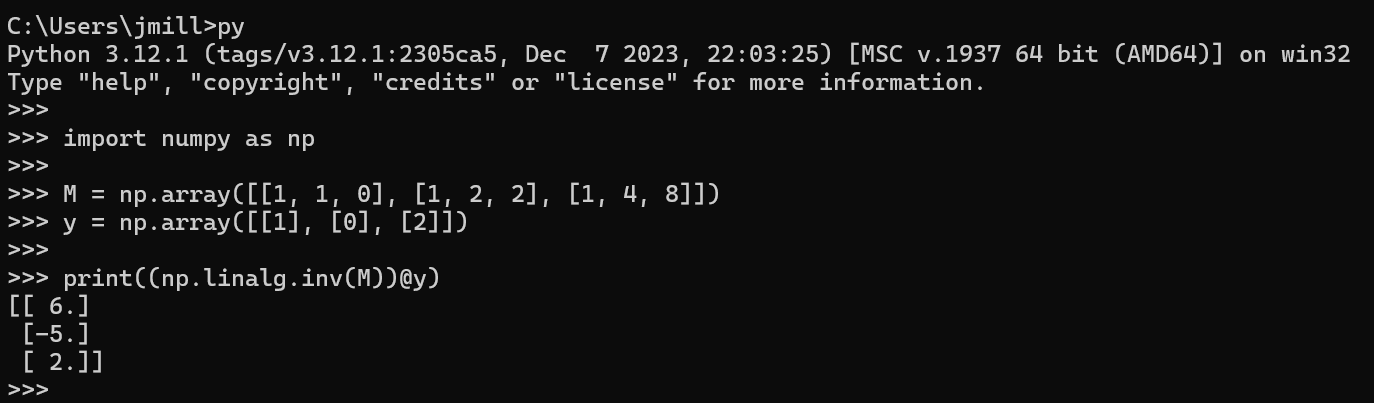
\includegraphics[scale=0.6]{188-HW1_Q1.png}\retTwo\par}

   So, $a_n = 6 - (5 + 2n)2^n$.\retTwo
\end{myIndent}

\blab{(2)} Let $(a_n)_{n\geq 0}$ and $(b_n)_{n \geq 0}$ be sequences. Assume that $(b_n)_{n \geq 0}$ satisfies a linear recurrence relation of order $e$. Then let $c_1, \ldots, c_d$ be scalars with $c_d \neq 0$ and assume that $(a_n)_{n \geq 0}$ satisfies:

{\centering $a_n = c_1a_{n-1} + \ldots + c_da_{n-d} + b_n$ for all $n \geq d$\retTwo\par}

Prove that $(a_n)_{n \geq 0}$ satisfies a linear recurrence relation of order $d + e$.

\begin{myIndent}\exOne
   To start, let's show some smaller facts:\retTwo

   \blab{Observation 1:} Suppose $a_n = c_1a_{n-1} + \ldots + c_da_{n-d} + p_m(n)r^n + F(n)$ where $F$ is some arbitrary function, $p_m$ is a polynomial of degree $m$ and $r$ is a nonzero constant. Then $a_n$ satisfies a recurrence relation of degree $e = d + m + 1$ where $F^\prime(n)$ is an arbitrary function $F(n)$ determined by $m$, $r$, and $F(n)$, and:
   
   {\centering $a_n = c^\prime_1 a_{n-1} + \ldots + c^\prime_e a_{n-e} + F^\prime(n)$ for all $n \geq e$.\newpage\par}
   
   \begin{myIndent}\exPP
         Proof by induction:\retTwo

         \blab{Lemma}: If $p_m(n)$ is a polynomial of degree $m > 0$, then $p_m(n) - p_m(n-1)$ is a\\ polynomial of degree $m - 1$.
         
         \begin{myIndent}\color{VioletRed}
            This is because for all $N > 0$ and coefficients $b$, we have that:\\ $bn^N - b(n - 1)^N = bn^N - bn^N + q(n)$ where $q$ is a polynomial\\ of degree $N - 1$. Meanwhile, the case where $N = 0$ is trivial.\retTwo
         \end{myIndent}

         \blab{Base Case:} If $m = 0$, meaning $p_m(n) = b$ where $b$ is a constant, then by taking the difference of $a_n$ and $r a_{n-1}$ for all $n \geq d + 1$, we get that:

         {\centering 
         \begin{tabular}{l}
            $a_n = (c_1 + r)a_{n-1} + (c_2 - rc_1)a_{n-2} + \ldots + (c_d - rc_{d-1})a_{n-d} - rc_da_{n-d-1}$\\ [4pt] $\phantom{Aaaaaaaaaaaaaaaaaaaaaaaaaaaaaaaaaaa} + F(n) - rF(n-1)$.
         \end{tabular} \retTwo\par}

         Setting $c_1^\prime = c_1 + 1, c_2^\prime = c_2 - rc_1,\phantom{.} \ldots,\phantom{.} c_d^\prime = c_d - rc_{d-1}, c_{d+1}^\prime = -rc_d$, and $F^\prime(n) = F(n) - rF(n - 1)$, we thus get that:

         {\centering$a_n = c_1^\prime a_{n-1} + \ldots + c_{d+1}^\prime a_{n-d-1} + F^\prime(n)$ for all $n \geq d + 1$.\par}
         
         \begin{myTindent}\begin{myDindent}\color{VioletRed}
            Also $c_{d+1}^\prime \neq 0$ because neither $r$ nor $c_d$ equal $0$.\retTwo
         \end{myDindent}\end{myTindent}

         
         \blab{Induction on $m$:} If $m > 0$, then by taking the difference of $a_n$ and $ra_{n-1}$ for all $n \geq d + 1$, since $r^n(p(n)) - rr^n(p(n-1)) = r^n(p(n) - p(n-1))$, we get by our lemma above that:\\ [-12pt]

         {\center
         \begin{tabular}{l}
            $a_n = (c_1 + r)a_{n-1} + (c_2 - rc_1)a_{n-2} + \ldots + (c_d - rc_{d-1})a_{n-d}$ \\ $\phantom{a_n = (c_1 + r)a_{n-1} + (c_2 - rc_1)a_{n-2}} - rc_da_{n-d-1} + q(n)r^n + F^\prime(n)$
         \end{tabular}\\ [6pt]\par}

         where $q$ is a polynomial of degree $m - 1$ and $F^\prime(n) = F(n) - rF(n-1)$.
         
         \begin{myDindent}\begin{myIndent}\color{VioletRed}
            And same as before, $-r c_d \neq 0$ because $r \neq 0$ and $c_d \neq 0$.\retTwo
         \end{myIndent}\end{myDindent}

         But now we can conclude by induction that $a_n$ satisfies a (possibly inhomogeneous) recurrence relation of order $e = (d + 1) + ((m - 1) + 1) = d + m + 1$ such that $F^\pprime(n)$ is some function determined by $m$, $r$ and $F(n)$, and:
         
         {\centering$a_n = c_1^\pprime a_{n-1} + \ldots + c_{e}^\pprime a_{n-e} + F^\pprime(n)$ for all $n \geq e$.\\ [26pt]\par}
   \end{myIndent}

   One important observation from above is that if $F(n) = 0$, then $F^\prime(n) = 0$. In some other situations, $F^\prime(n)$ also behaves nicely.\retTwo

   \blab{Observation 2:} Let $p_1(n), \ldots, p_k(n)$ be polynomials of degree $m_1, \ldots, m_k$ respectively. Also let $r_1, \ldots r_k$ be distinct nonzero constants. If:
   
   {\centering $a_n = c_1a_{n-1} + \ldots + c_da_{n-d} + p_1(n)r_1^n + F(n)$\\ \par}

   where $F(n) = \sum\limits_{i=2}^k p_i(n)r_i^n$, then part 1 will make  $F^\prime(n) = \sum\limits_{i = 2}^k q_i(n)r_i^n$ where\\ $q_2(n), \ldots, q_k(n)$ are also polynomials of degree $m_2, \ldots, m_k$ respectively.\\ [-6pt]

   \begin{myIndent}\exPP
      To see why, note that:
      
      {\centering $F(n) - r_1F(n -1) = \sum\limits_{i =2}^k p_i(n)r_i^n - \sum\limits_{i = 2}^k p_i(n - 1)r_1r_i^{n-1}$ \\
      $\phantom{F(n) - r_1F(n -1) = \sum\limits_{i =2}^k p_i(n)r_i^n} = \sum\limits_{i = 2}^k (p_i(n) - \frac{r_1}{r_i}p_i(n - 1))r_i^n$ \newpage\par}

      Because $r_i \neq r_1$, we know $\frac{r_1}{r_i} \neq 1$, meaning that the degree $m$ term of\\ $p_i(n) - \frac{r_1}{r_i}p_i(n - 1)$ doesn't cancel. So $q_i(n) \coloneq p_i(n) - \frac{r_1}{r_i}p_i(n - 1)$\\ is still a degree $m$ polynomial. If the process in part 1 takes more steps, then\\ we can just repeat this reasoning.\\ [6pt]
   \end{myIndent}

   Combining observations 1 and 2 together, we can inductively show that if
   
   {\centering $a_n = c_1a_{n-1} + \ldots + c_da_{n-d} + \sum\limits_{i = 1}^k p_i(n)r_i^n$\par}

   where $r_1, \ldots, r_k$ are distinct nonzero constants and $p_1(n), \ldots, p_k(n)$\\ [-6pt] are polynomials of degree $m_1, \ldots, m_k$ respectively, then letting $e = \sum\limits_{i=1}^k(m_i + 1)$,\\ [-6pt] there exists constants $c_1^\prime, \ldots c_{d + e}^\prime$ such that:

   {\centering $a_n = c_1^\prime a_{n-1} + \ldots + c_{e+d}^\prime a_{n-d-e}$ \retTwo\par}

   But now note that if $(b_n)_{n \geq 0}$ satisfies a linear recurrence relation of order $e$, we\\ [-2pt] can write $b_n = \sum\limits_{i = 1}^k p_i(n)r_i^n$ for some polynomials $p_1(n),\ldots p_k(n)$ with degrees\\ [-2pt] $m_1, \ldots, m_k$, as well as some distinct nonzero constants $r_1, \ldots, r_k$.
   
   \begin{myTindent}\exPP
      We know that each $r_i$ is nonzero because the constant term in the characteristic polynomial for $(b_n)$'s recurrence relation must be nonzero.\retTwo
   \end{myTindent}

   Also, as we showed in class, $\sum\limits_{i = 1}^k(m_i + 1) = e =$ the order of the recurrence relation\\ [-6pt] of $(b_n)_{n \geq 0}$.\retTwo

   So, we've shown that $a_n = c_1a_{n-1} + \ldots + c_da_{n-d} + b_n$ can be rewritten as a\\ homogenous linear recurrence relation of order $(d + e)$.\retTwo
\end{myIndent}

\blab{(3)} Let $(f_n)_{n \geq 0}$ be the Fibonacci numbers, and define $a_n = \sum\limits_{i = 0}^n f_i$.
\begin{itemize}
   \item[(a)] Find a linear recurrence relation of order $3$ that $(a_n)_{n \geq 0}$ satisfies.
   
   \begin{myIndent}\exOne
      Note that $(a_n)_{n \geq 0}$ satisfies the relation $a_n = a_{n - 1} + f_n$ for all $a_n$. Also, we showed in the first lecture that:

      {\centering $f_n = \frac{1}{\sqrt{5}}\left(\frac{1 + \sqrt{5}}{2}\right)^n - \frac{1}{\sqrt{5}}\left(\frac{1 - \sqrt{5}}{2}\right)^n $ \retTwo\par}

      So we know that: $a_n = a_{n-1} + \frac{1}{\sqrt{5}}\left(\frac{1 + \sqrt{5}}{2}\right)^n - \frac{1}{\sqrt{5}}\left(\frac{1 - \sqrt{5}}{2}\right)^n$\hspace{-0.4em}.

      Firstly, taking the difference of $a_n$ and $\frac{1 + \sqrt{5}}{2}a_{n-1}$, after a lot of simplifying we have that:
      
      \begin{myIndent}\exPP
         \begin{tabular}{l}
            $a_n = (1 + \frac{1 + \sqrt{5}}{2})a_{n-1} - \frac{1 + \sqrt{5}}{2}a_{n-2} + \left(-\frac{1}{\sqrt{5}} + \frac{1 + \sqrt{5}}{2\sqrt{5}}\cdot\frac{2}{1 - \sqrt{5}}\right)\left(\frac{1 - \sqrt{5}}{2}\right)^{n}$\\ [8pt]
            $\phantom{a_n} = \frac{3 + \sqrt{5}}{2}a_{n-1} - \frac{1 + \sqrt{5}}{2}a_{n-2} + \left(\frac{1 - \sqrt{5}}{2}\right)^{n-1}$
         \end{tabular}\newpage
      \end{myIndent}

      Secondly, we take the difference of $a_n$ and $\frac{1 - \sqrt{5}}{2}a_{n-1}$, and after a lot more\\ simplifying get:

      \begin{myIndent}\exPP
         \begin{tabular}{l}
            $a_n = \left(\frac{3 + \sqrt{5}}{2} + \frac{1-\sqrt{5}}{2}\right)a_{n-1} - \left(\frac{1 + \sqrt{5}}{2} + \frac{1-\sqrt{5}}{2}\cdot \frac{3+\sqrt{5}}{2}\right)a_{n-2} + \left(\frac{1-\sqrt{5}}{2}\cdot\frac{1 + \sqrt{5}}{2}\right)a_{n-3}$ \\ [8pt]
            $\phantom{a_n} = 2a_{n-1} + 0a_{n-2} - a_{n-3}$
         \end{tabular}\retTwo
      \end{myIndent}
   \end{myIndent}

   \item[(b)] Find a closed formula for $a_n$. 
   
   \begin{myIndent}\exOne
      \blab{Method 1:}\\
      The characteristic polynomial of $a_n = 2a_{n-1} - a_{n-3}$ is $t^3 - 2t^2 + 1$. Just by looking at it, I can already see that $(t - 1)$ is a factor of that polynomial. So after doing polynomial long division, we have that $(t - 1)(t^2 - t - 1) = t^3 - 2t^2 + 1$.\retTwo

      By quadratic formula, the remaining roots are $\frac{1 + \sqrt{5}}{2}$ and $\frac{1 - \sqrt{5}}{2}$ (a.k.a the same roots as with the Fibonacci recurrence relation).\retTwo

      Finally, we get a system of linear equations:
      
      {\centering$
      \begin{bmatrix}
         1 & 1 & 1 \\ 1 & \frac{1 + \sqrt{5}}{2} & \frac{1 - \sqrt{5}}{2} \\  1 & \left(\frac{1 + \sqrt{5}}{2}\right)^2 & \left(\frac{1 - \sqrt{5}}{2}\right)^2
      \end{bmatrix}
      \begin{bmatrix}
         \beta_1 \\ \beta_2 \\ \beta_3
      \end{bmatrix} = 
      \begin{bmatrix}
         0 \\ 1 \\ 2
      \end{bmatrix}$\retTwo\par}

      To solve this, I finally started learning sympy:

      {\centering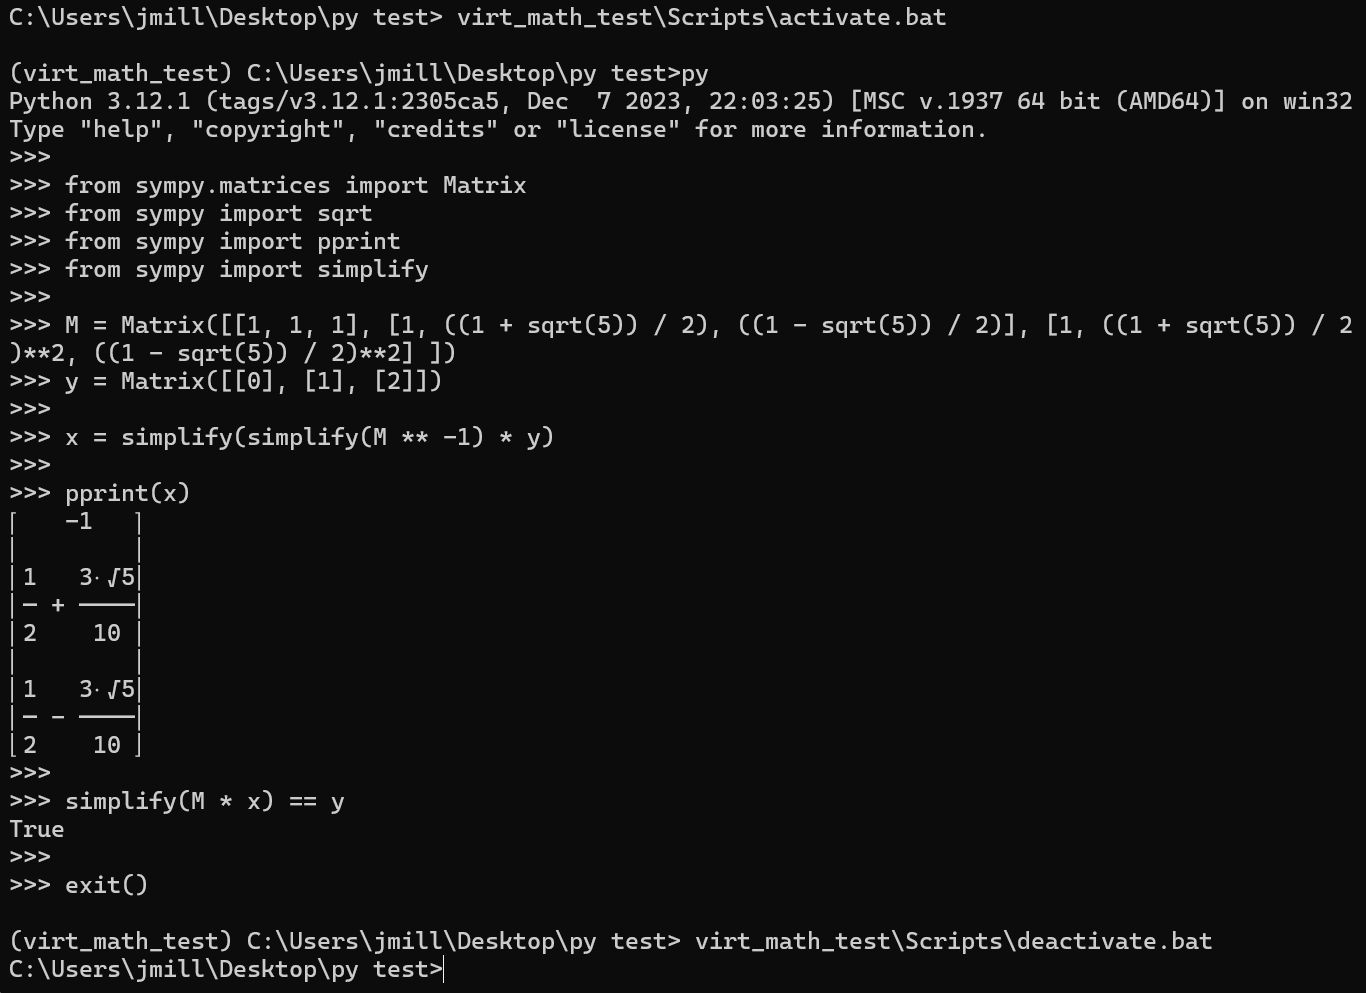
\includegraphics[scale=0.58]{188-HW1_Q3.png}\newpage\par}

      So, assuming I've not made a silly error somewhere, we should have that:

      {\centering $a_n = -1 + \left(\frac{5 + 3\sqrt{5}}{10}\right)\left(\frac{1 + \sqrt{5}}{2}\right)^n + \left(\frac{5 - 3\sqrt{5}}{10}\right)\left(\frac{1 - \sqrt{5}}{2}\right)^n$ \retTwo\par}

      \blab{Method 2: (The hinted route)}\\
      Note that $\frac{1 - r^{n+1}}{1-r} = \sum\limits_{i=0}^n r^i$. Using this fact, we can see that:

      {\centering\exPP
      \begin{tabular}{l}
         $a_n = \sum\limits_{i = 0}^n f_i = \frac{1}{\sqrt{5}}\sum\limits_{i = 0}^n\left(\frac{1 + \sqrt{5}}{2}\right)^i - \frac{1}{\sqrt{5}}\sum\limits_{i = 0}^n\left(\frac{1 - \sqrt{5}}{2}\right)^i$ \\ [10pt]
         $\phantom{a_n = \sum\limits_{i = 0}^n f_i} = \frac{1}{\sqrt{5}}\cdot \frac{1}{1 - \frac{1 + \sqrt{5}}{2}}\left(1 - (\frac{1 + \sqrt{5}}{2})^{n + 1}\right) - \frac{1}{\sqrt{5}}\cdot \frac{1}{1 - \frac{1 - \sqrt{5}}{2}}\left(1 - (\frac{1 - \sqrt{5}}{2})^{n + 1}\right)$
      \end{tabular}\retTwo\par}

      Now technically we are done since that is a closed formula for $a_n$. However, it looks ugly. So I'm going to learn more sympy so it can symplify this:

      {\centering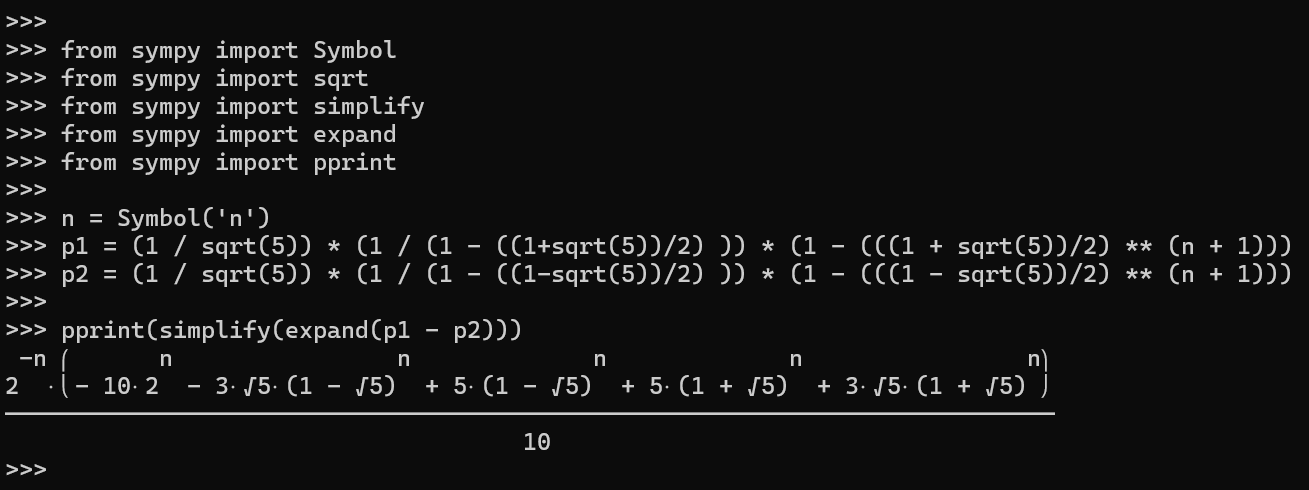
\includegraphics[scale=0.58]{188-HW1_Q3B.png}\retTwo\par}

      Hence we get the same answer as before:

      {\centering $a_n = -1 + \left(\frac{5 + 3\sqrt{5}}{10}\right)\left(\frac{1 + \sqrt{5}}{2}\right)^n + \left(\frac{5 - 3\sqrt{5}}{10}\right)\left(\frac{1 - \sqrt{5}}{2}\right)^n $ \retTwo\par}
   \end{myIndent}
\end{itemize}

\blab{(4)}
\begin{enumerate}
   \item[(a)] Suppose that $(a_n)_{n \geq 0}$ and $(a_n^\prime)_{n \geq 0}$ both satisfy the same linear recurrence\\ relation of order $d$ and that they agree in $d$ consecutive places, i.e. there exists $k$ such that $a_k = a^\prime_k$, $a_{k+1} = a^\prime_{k+1}$, \dots, $a_{k+d-1} = a^\prime_{k+d-1}$. Then these sequences are the same.
   
   \begin{myIndent}\exOne
      This is because for all integers $N \geq 0$ and sequences $(b_n)_{n \in \mathbb{Z}}$ satisfying a linear\\ recurrence relation: $b_n = c_1b_{n-1} + \ldots + c_db_{n-d}$ for all integers $n \geq d$, we have that:
         
      {\centering 
      \begin{tabular}{c}
         $N + d \geq d$ \\ $\left.\vphantom{\int}\right\Downarrow$ \\ $b_{N+d} = c_1b_{N + d - 1} + \ldots + c_{d-1}b_{N + 1} + c_db_{N}$\\ $\left.\vphantom{\int}\right\Updownarrow$ \\ $b_N = \frac{1}{c_d}b_{N + d} - \frac{c_1}{c_d}b_{N + d - 1} - \ldots - \frac{c_{d-1}}{c_d}b_{N + 1}$
      \end{tabular} \newpage\par}

      Now suppose we know $d$ consecutive elements of $(b_n)_{n \geq 0}$ (say $b_{k}$, $b_{k + 1}$, \ldots,\\ and $b_{k + d -1}$ where $k$ is a nonnegative integer). Then we can uniquely solve\\ for $b_n$ by inductively applying our recurrence relation when $n > k + d - 1$.\\ Plus, we can uniquely solve for $b_n$ by inductively using the identity we\\ found on the previous page when $n < k$. So $(b_n)_{n \geq 0}$ is uniquely determined by its consecutive elements $b_{k}$, $b_{k + 1}$, \ldots, and $b_{k + d -1}$. \retTwo

      Since $(a_n)_{n \geq 0}$ and $(a_n^\prime)_{n \geq 0}$ are uniquely determined by the same consecutive elements, we thus know that the sequences are the same.\retTwo
   \end{myIndent}

   \item[(b)] Suppose that $(a_n)_{n \geq 0}$ satisfies the linear recurrence relation of order $d$:\\ $a_n = c_1a_{n-1} + \ldots + c_da_{n-d}$ for all $n \geq d$. Then there is a unique sequence $(b_n)_{n \in \mathbb{Z}}$ such that $b_n = a_n$ for $n \geq 0$ and $b_n = c_1b_{n-1} + \ldots + c_db_{n-d}$ for all\\ $n \in \mathbb{Z}$.
   
   \begin{myIndent}\exOne
      If $N < 0$, we can still inductively apply the identity we found on the last\\ [2pt] page: $b_N = \frac{1}{c_d}b_{N + d} - \frac{c_1}{c_d}b_{N + d - 1} - \ldots - \frac{c_{d-1}}{c_d}b_{N + 1}$ in order to uniquely solve\\ [3pt] for $b_N$ such that $b_{N + d} = c_1b_{N + d - 1} + \ldots + c_db_{N}$.\retTwo

      Hence, given a sequence $(a_n)_{n \geq 0}$ satisfying a linear recurrence relation of order $d$: $a_n = c_1a_{n-1} + \ldots + c_da_{n-d}$, we define $b_n = a_n$ when $n \geq 0$. Meanwhile, when $n < 0$, we inductively define $b_n$ as:
      
      {\centering $b_n = \frac{1}{c_d}b_{n + d}- \frac{c_1}{c_d}b_{n + d - 1} - \ldots - \frac{c_{d-1}}{c_d}b_{n + 1}$.\retTwo\par}

      Then $(b_n)_{n \in \mathbb{Z}}$ is the unique sequence satisfying the problem's requirements.\retTwo
   \end{myIndent}

   \item[(c)] Consider the Fibonacci sequence $(f_n)_{n \geq 0}$. How does the negatively indexed Fibonacci sequence relate to the usual one?
   
   \begin{myIndent}\exOne
      If $f_{n+2} = f_{n+1} + f_{n}$, then we know $f_{n} = - f_{n+1} + f_{n + 2}$. Defining $g_{n} = f_{-n}$, we thus get the recurrence relation: $g_n = -g_{n-1} + g_{n-2}$, and its characteristic polynomial is $t^2 + t - 1$.\retTwo

      Now let $r_1$ and $r_2$ be the roots of $t^2 - t - 1$, the characteristic polynomial of $f_n$. Then subbing in $t = (-s)$, we get that:

      {\centering $t^2 - t - 1 = (t - r_1)(t - r_2) \Longrightarrow s^2 + s - 1 = (s + r_1)(s + r_2)$\retTwo\par}

      So, there exists constants $\alpha_1, \alpha_2$ such that:
      
      {\centering $g_n = \alpha_1(-1)^n\left(\frac{1+\sqrt{5}}{2}\right)^n + \alpha_2(-1)^n\left(\frac{1-\sqrt{5}}{2}\right)^n$.\retTwo\par}

      Since $g_{1} = f_{-1} = -f_0 + f_1 = 1$ and $g_0 = f_0 = 0$, by plugging in $n = 0$ and $n = 1$, we get the following matrix equation:

      {\centering $\begin{bmatrix}
         1 & 1 \\ -\frac{1+\sqrt{5}}{2} & -\frac{1-\sqrt{5}}{2}
      \end{bmatrix}
      \begin{bmatrix}
         \alpha_1 \\ \alpha_2
      \end{bmatrix} = 
      \begin{bmatrix}
         0 \\ 1
      \end{bmatrix}$\newpage\par}

      After solving that, we get that $\alpha_1 = \frac{-1}{\sqrt{5}}$ and $\alpha_2 = \frac{1}{\sqrt{5}}$ So in conclusion:

      {\centering $f_{-n} = g_n = \frac{1}{\sqrt{5}}(-1)^{n+1}\left(\frac{1+\sqrt{5}}{2}\right)^n - \frac{1}{\sqrt{5}}(-1)^{n+1}\left(\frac{1-\sqrt{5}}{2}\right)^n = (-1)^{n+1} f_n$ \retTwo\par}

      
      \begin{myTindent}\exPP\color{VioletRed}
         I could have probably proven the identity $f_{-n} = (-1)^{n+1} f_n$\\ much faster by just doing induction and assuming\\ $f_{-N} = (-1)^{N+1} f_N$ for all $N \in \{0, 1, \ldots, n-1\}$.\retTwo
      \end{myTindent}
   \end{myIndent}
\end{enumerate}

\blab{(5)} Let $p$ be a prime number and let $(a_n)_{n \geq 0}$ be a sequence such that $a_n \in \mathbb{Z}_p$ and which satisfies a homogeneous linear recurrence relation. Prove that the sequence is periodic, i.e. there exists $N$ such that $a_n = a_{n + N}$ for all $n \geq 0$.\\ [-10pt]

\begin{myIndent}\exOne
   Consider the set $\{(a_n, a_{n+1},\ldots, a_{n+d-1}) \mid n \in \mathbb{Z} \text{ and } n \geq 0\}$. Then note that it is a subset of $(\mathbb{Z}_p)^d$ which is finite with $p^d$ elements. Hence, given some $(\beta_0, \ldots, \beta_d)$ in that set, we know there exists infinitely many $n \geq 0$ such that:

   {\centering$(a_n, a_{n+1},\ldots, a_{n+d-1}) = (\beta_0, \beta_1, \ldots, \beta_{d-1})$.\retTwo\par} 
   
   Let $S$ be the set of all such $n$. Then pick $n_1$ and $n_2$ to be the least and second least elements of $S$ respectively. We claim $(a_n)_{n \geq 0}$ is periodic with period $N = n_2 - n_1$.\retTwo

   \begin{myIndent}\exTwoP
      Firstly, we'll prove by induction that $a_n = a_{N + n}$ when $n \geq n_1$. For our\\ base case, we know from how we picked $n_1$ and $n_2$ that $a_n = a_{N + n}$ when\\ $n_1 \leq n < n_1 + d$. Meanwhile, suppose that given some $k \geq d$ we have that\\ $a_n = a_{N + n}$ for all $n_1 \leq n < n_1 + k$. Then using our recurrence relation, when we solve for $a_k$ and $a_{k + N}$, we will get that they are equal. Hence, we know by induction that $a_n = a_{n + N}$ for all $n \geq n_1$.\retTwo

      Next, consider that if $a_n = c_1a_{n-1} + \ldots + c_d a_{n-d}$ for all $n \geq d$, then for all $n \geq 0$ we have that: $a_n = \frac{1}{c_d}a_{n + d} - \frac{c_1}{c_d}a_{n + d - 1} - \ldots - \frac{c_{d-1}}{c_d}a_{n + 1}$.
      
      \begin{myTindent}\exPP\color{VioletRed}
         This expression is still well-defined in $\mathbb{Z}_p$ because $c_d \neq 0$ and all nonzero elements in $\mathbb{Z}_p$ have a multiplicative inverse since $p$ is prime.\retTwo
      \end{myTindent}

      Thus, we can proceed by induction to show that $a_n = a_{N + n}$ for all $n \geq 0$.\\ Our base case is that if $n \geq n_1$, we know from before that $a_n = a_{n + N}$.\\ Meanwhile, suppose that given some $k < d$ we have that $a_n = a_{n + N}$ for\\ all $n > k$. Then when we use the expression above to calculate $a_k$ and $a_{k + N}$, we will get that they equal each other. Hence, we know by induction that $a_n = a_{n + N}$ for all nonnegative integers $n$.\retTwo
   \end{myIndent}
\end{myIndent}

\mySepTwo

\newpage

\mHeader{Homework 2:}

\blab{(1)} Let $A(x)$ be a formal power series with $A(0) = 0$.\\ [-20pt]
\begin{enumerate}
   \item[(a)] Show that there exists a formal power series $B(x)$ with $B(0) = 0$ such that\\ $A(B(x)) = x$ if and only if $[x^1]A(x) \neq 0$.
   
   \begin{myIndent}\exOne
      Let us write $A(x) = \sum\limits_{n \geq 1}a_nx^n$ and $B(x) = \sum\limits_{n \geq 1}b_nx^n$.\\ [-6pt]
      
      \begin{myTindent}\exPP
         We start indexing at $1$ because we know from the problem\\ statement that $a_0 = 0$, and $A(B(x))$ is not defined unless\\ $b_0 = 0$.\retTwo
      \end{myTindent}

      Note that $[x^1]A(B(x)) = a_1b_1$. So if $a_1 = [x^1]A(x) = 0$, then we can't solve for $b_1$ such that $a_1b_1 = 1$. On the other hand, if $a_1 \neq 0$ (a.k.a it has a multiplicative inverse), then we can uniquely fix $b_1 = \sfrac{1}{a_1}$.\retTwo

      After that, note that for any $n \in \mathbb{Z}_{\geq 2}$, we have that:
      
      {\centering $[x^n]A(B(x)) = a_1b_n + f_{a_2, \ldots, a_{n}, b_1,\ldots, b_{n-1}}$\par}
      
      where the end term is some expression of given coefficients and coefficients which we can calculate by induction. So, forcing $[x^n]A(B(x)) = 0$, we can\\ uniquely determine $b_n$ to be:

      {\centering $b_n = -\frac{1}{a_1}f_{a_2, \ldots, a_{n}, b_1,\ldots, b_{n-1}}$ \retTwo\par}

      \begin{myIndent}\exPP
         To better explain why the coefficients of $A(B(x))$ take on the form above,\\ note that $\mdeg A(x) = 1 \Longrightarrow \mdeg A(x)^n \geq n$. Also, if $B(x)$ with\\ $B(0) = 0$ is raised to a power $m \geq 2$, then the first coefficient which $[x^n]B(x)$ will affect in $[x^n]B(x)^m$ is $[x^{m + n - 1}]B(x)^m$.\retTwo
      \end{myIndent}

      It follows that by induction, there exists a unique formal power series $B(x)$ such that $A(B(x)) = x$.\retTwo
   \end{myIndent}

   \item[(b)] Assuming $[x^1]A(x) \neq 0$, show that $B(x)$ is unique and also satisfies\\ $B(A(x)) = x$. You may use without proof that composition of formal\\ power series is associative.
   
   \begin{myIndent}\exOne
      We know from before that $B(x)$ is unique. Meanwhile, note that if\\ $(A \circ B)(x) = x$ and composition is associative, then:
      
      {\centering $(A \circ B)(A(x)) = A(x) \Longrightarrow A((B \circ A)(x)) = A(x) \Longrightarrow (B \circ A)(x) = x$ \retTwo\par}
      
      \begin{myIndent}\exPP
         Actually, to be fully rigorous I still need to show that:
         
         {\centering $A(B(x)) = A(C(x)) \Longrightarrow B(x) = C(x)$\phantom\retTwo\par}

         
         \begin{myTindent}
            \exPPP I'll write this after question 5 since I didn't notice I needed to do this until rather late.
         \end{myTindent}
      \end{myIndent}
   \end{myIndent}
\end{enumerate}

\blab{(2)} 
\begin{enumerate}
   \item[(a)] Prove that $\hspace{-0.25em}\sum\limits_{m,n \geq 0}\hspace{-0.25em}\min(m,n)x^my^n = \frac{xy}{(1-x)(1-y)(1-xy)}$.
   
   \begin{myIndent}\exOne
      Firstly, note that $\hspace{-0.25em}\sum\limits_{m,n \geq 0}\hspace{-0.25em}\min(m,n)x^my^n = \sum\limits_{m \geq 0}\left(\sum\limits_{n=0}^{m}ny^n + \sum\limits_{n > m}my^n\right)x^m$.\retTwo

      Also, we have that:
      \begin{itemize}
         \item $\sum\limits_{n > m}m y^n = my^{m + 1} \sum\limits_{n \geq 0}y^n = \frac{my^{m+1}}{1 - y}$.
         \item $\sum\limits_{n=0}^m ny^n = y\sum\limits_{n=0}^{m-1} (n+1)y^{n}$\\
         $\phantom{\sum\limits_{n=0}^m ny^n } = yD\hspace{-0.2em}\left(\sum\limits_{n=0}^m y^n\right) = yD\left(\frac{1 - y^{m+1}}{1- y}\right)$\\
         $\phantom{\sum\limits_{n=0}^m ny^n = yD\hspace{-0.2em}\left(\sum\limits_{n=0}^m y^n\right)} = y\left(\frac{-(m + 1)y^m}{1 - y} + \frac{1 - y^{m+1}}{(1-y)^2}\right) = \frac{-my^{m+1} - y^{m+1}+my^{m+2}+y}{(1-y)^2}$\retTwo
      \end{itemize}

      Thus, $\sum\limits_{n=0}^{m}ny^n + \sum\limits_{n > m}my^n = \frac{y - y^{m+1}}{(1-y)^2}$.\retTwo

      And therefore:
      
      {\centering 
      \begin{tabular}{l}
         $\sum\limits_{m,n \geq 0}\hspace{-0.25em}\min(m,n)x^my^n = \frac{y}{(1-y)^2}\sum\limits_{m \geq 0}(1 - y^m)x^m$\\ [14pt]
         $\phantom{\sum\limits_{m,n \geq 0}\hspace{-0.25em}\min(m,n)x^my^n} = \frac{y}{(1-y)^2}\sum\limits_{m \geq 0}x^m - \frac{y}{(1-y)^2}\sum\limits_{m \geq 0}x^my^m$\\ [14pt]
         $\phantom{\sum\limits_{m,n \geq 0}\hspace{-0.25em}\min(m,n)x^my^n} = \frac{y}{(1-y)^2}\cdot\frac{1}{1-x} - \frac{y}{(1-y)^2}\cdot\frac{1}{1-xy}$\\ [2pt]
         $\phantom{\sum\limits_{m,n \geq 0}\hspace{-0.25em}\min(m,n)x^my^n} = \frac{-xy^2 + xy}{(1-y)^2(1-x)(1-xy)} = \frac{xy}{(1-y)(1-x)(1-xy)}$
      \end{tabular}\retTwo\par}
   \end{myIndent}
   
   \item[(b)] Let $a_{m,n}$ be the number of paths in $\mathbb{R}^2$ from $(0, 0)$ to $(m, n)$ using steps of the form $\overrightarrow{(1, 0)}$, $\overrightarrow{(0, 1)}$, and $\overrightarrow{(2, 1)}$. Prove that:
   
   {\centering $\sum\limits_{m,n\geq 0}\hspace{-0.25em}a_{m,n}x^my^n = \frac{1}{1-x-y-x^2y}$ \retTwo\par}

   
   \begin{myIndent}\exOne
      Note that for $m \geq 2$ and $n \geq 1$, we have that:
      
      {\centering $a_{m,n} = a_{m-1, n} + a_{m, n-1} + a_{m-2, n-1} $ \retTwo\par}
   
      Also, we can somewhat trivially calculate that $a_{m, 0} = 1 = a_{0, n}$ if $m, n > 0$, that $a_{1, n} = n+1$ if $n \geq 0$, and that $a_{0,0} = 1$ (the empty path). Thus:
      \begin{itemize}
         \item $m \geq 1 \Longrightarrow [x^m](1 - x - y - x^2y)A(x) = a_{m,0} - a_{m-1, 0} = 0$
         \item $n \geq 1 \Longrightarrow [y^n](1 - x - y - x^2y)A(x) = a_{0,n} - a_{0, {n-1}} = 0$
         \item $n \geq 1 \Longrightarrow [xy^n](1 - x - y - x^2y)A(x) = a_{1, n} - a_{0, n} - a_{1, n-1} = 0$\newpage
         \item $[x^0y^0](1 - x - y - x^2y)A(x) = a_{0,0} = 1$.
      \end{itemize}

      Thus,  $(1 - x - y - x^2y)A(x) = 1$. And so $A(x) = \frac{1}{1 - x - y - x^2y}$.\retTwo
   \end{myIndent}
\end{enumerate}

\blab{(3)} Let $n \geq 2$ be an integer. Evaluate the following sums:

\begin{enumerate}
   \item[(a)] $\sum\limits_{i=0}^n i^2\binom{n}{i}$
   
   \begin{myIndent}\exOne
      Note that by taking derivatives of the binomial theorem, we get that:\\ [-18pt]
      {\exTwo\begin{itemize}
         \item $n(x+1)^{n-1} = \sum\limits_{i=1}^{n} i\binom{n}{i}x^{i-1}$
         \item $ n(n-1)(x+1)^{n-2} = \sum\limits_{i=2}^{n} i(i-1)\binom{n}{i} x^{i-2} = \sum\limits_{i=2}^ni^2\binom{n}{i}x^{i-2} - \sum\limits_{i=2}^ni\binom{n}{i}x^{i-2}$\retTwo
      \end{itemize}}

      So, since $i\binom{n}{i}x^{i} = i^2\binom{n}{i}x^{i}$ when $i = 0$ or $i = 1$, we can multiply everything by $x^2$ rearrange terms, and then add the missing terms to both sides to get that:
      
      {\centering 
      \begin{tabular}{l}
         $\sum\limits_{i=0}^n i^2\binom{n}{i}x^i = n(n-1)x^2(x+1)^{n-2} + x\sum\limits_{i=0}^n i\binom{n}{i}x^{i-1}$\\ $\phantom{\sum\limits_{i=0}^n i^2\binom{n}{i}x^i}= n(n-1)x^2(x+1)^{n-2} + nx(x+1)^{n-1}$
      \end{tabular}\retTwo\par}

      Subbing in $x = 1$, we thus get that:
      
      {\centering $\sum\limits_{i=0}^n i^2\binom{n}{i} = (n(n-1) + 2n)2^{n-2} = (n^2 + n)2^{n-2}$.\retTwo\par}
   \end{myIndent}

   \item[(b)] $\sum\limits_{i=0}^n i^2\binom{n}{i}(-1)^i$
   
   \begin{myIndent}\exOne
      Starting back off with the expression for $\sum\limits_{i=0}^n i^2\binom{n}{i}x^i$ we found last time, we instead sub in $x = -1$ to get that:

      {\centering $\sum\limits_{i=0}^n i^2\binom{n}{i}(-1)^ix^i = n(n-1)x^2(1-x)^{n-2} - nx(1-x)^{n-1}$ \retTwo\par}



      Interestingly, if $n > 2$, then when we plug in $x = 1$, everything cancels and we get $\sum\limits_{i=0}^n i^2\binom{n}{i}(-1)^i = 0$. Meanwhile, if $n = 2$, then $(1 - x)^{n-2}$ doesn't equal zero and we get that:

      {\centering $\sum\limits_{i=0}^n i^2\binom{n}{i}(-1)^i = 2$ \newpage\par}
   \end{myIndent}

   \item[(c)] $\sum\limits_{
   \begin{smallmatrix}
      0 \leq i \leq n \\
      i \text{ is even}
   \end{smallmatrix}} \hspace{-0.6em}i^2\binom{n}{i}$

   \begin{myIndent}\exOne
      Combining the two previous sums, we get that:

      {\centering $\sum\limits_{
   \begin{smallmatrix}
      0 \leq i \leq n \\
      i \text{ is even}
   \end{smallmatrix}} \hspace{-0.6em}i^2\binom{n}{i} = \frac{1}{2}\sum\limits_{i=0}^n i^2\binom{n}{i} + \frac{1}{2}\sum\limits_{i=0}^n i^2\binom{n}{i}(-1)^i = \left\{
   \begin{matrix}
      (n^2 + n)2^{n-3} & \text{ if } n > 2 \\
      4 & \text{ if } n = 2
   \end{matrix}\right.$\retTwo\par}
   \end{myIndent}

   \item[(d)] $\sum\limits_{\begin{smallmatrix}
      0 \leq i \leq n \\
      i \text{ is odd}
   \end{smallmatrix}} \hspace{-0.6em}i^2\binom{n}{i}$

   \begin{myIndent}\exOne
      Combining the sum in part (a) and the sum in part (c), we get that:

      {\centering $\sum\limits_{
   \begin{smallmatrix}
      0 \leq i \leq n \\
      i \text{ is odd}
   \end{smallmatrix}} \hspace{-0.6em}i^2\binom{n}{i} = \sum\limits_{i=0}^n i^2\binom{n}{i} - \hspace{-0.6em} \sum\limits_{
      \begin{smallmatrix}
         0 \leq i \leq n \\
         i \text{ is even}
      \end{smallmatrix}} \hspace{-0.6em}i^2\binom{n}{i} = \left\{
   \begin{matrix}
      (n^2 + n)2^{n-3} & \text{ if } n > 2 \\
      2 & \text{ if } n = 2
   \end{matrix}\right.$\retTwo\par}
   \end{myIndent}
\end{enumerate}

\blab{(4)}
\begin{enumerate}
   \item[(a)] How many ways can we rearrange the letters of the word "SASSAFRAS"?
   
   \begin{myIndent}\exOne
      Something I'd briefly like to note is that an obvious upper bound for this\\ number is $9! = 362880$. Now while this bound does overcount (by quite a lot) since it isn't taking into account repeating letters, it is a small enough that you could write a snippet of code to manually count up this quantity. In fact, I did write some code to do that and preemptively got back that the answer is $2520$.\retTwo

      {\centering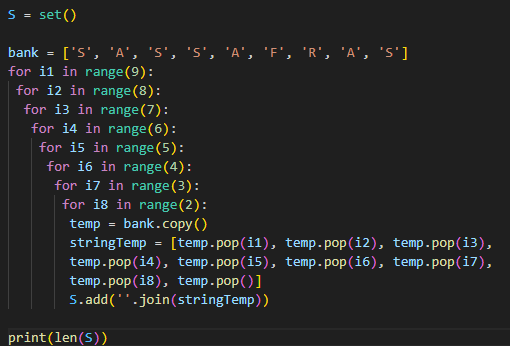
\includegraphics[scale=0.75]{188-HW2_Q4a.png}\retTwo\par}

      Now, consider the expansion of the polynomial: $(s + a + f + r)^9$. Given any string of nine letters: 's', 'a', 'f', 'r', we can associate that string with the term in the expansion gained by choosing to multiply in the $i$th letter of the string at step $i$.\retTwo

      It follows that $[s^4a^3fr](s + a + f + r)^9$ equals the number terms in the expansion associated with strings which rearrange the letters of "SASSAFRAS". And, we know that:

      {\centering\exP $[s^4a^3fr](s + a + f + r)^9 = \binom{9}{4, 3, 1, 1} = \frac{9!}{4!3!} = \frac{9\cdot 8 \cdot 7 \cdot 6 \cdot 5}{3 \cdot 2} = 9\cdot 8\cdot 7 \cdot 5 = 2520$ \newpage\par}
   \end{myIndent}

   \item[(b)] How many ways can this be done if we also require that the 3 A's all appear consecutively?
   
   \begin{myIndent}\exOne
      After modifying my code from before, I preemptively know that the right\\ answer is $210$. So, whatever we do next, our final answer should match that.\retTwo

      Now forcing all three A's to be next to each other means that whenever we choose A from among our bank of possible letters, we have to add A three times. The generating function that models this pattern of choosing letters is:
      
      {\centering $(s + (a^3) + f + r)^7 = \sum \binom{7}{k_1, k_2, k_3, k_4}s^{k_1}(a^3)^{k_2}f^{k_3}r^{k_4}$  \retTwo\par}

      Importantly, $[s^4a^3fr](s + a^3 + f + r)^7$ will still give the number of ways to arrange the letters of "SASSAFRAS". However, now:

      {\centering $[s^4a^3fr](s + a^3 + f + r)^7 = \binom{7}{4, 1, 1, 1} = 7\cdot6\cdot 5 = 210$\retTwo\par}
   \end{myIndent}
\end{enumerate}

\blab{(5)}
\begin{enumerate}
   \item[(a)] Let $a, b$ be rational numbers. Show that for any formal power series $A(x)$ with $A(0) = 1$, we have $A(x)^aA(x)^b = A(x)^{a + b}$.
   
   \begin{myIndent}\exOne
      To start, here's the proof that if $n,m, c$ are integers with $c \neq 0$, then\\ $A(x)^{\frac{m}{n}} = A(x)^{\frac{cm}{cn}}$:

      {\centering\exP  $(A(x)^{\sfrac{1}{cn}})^{cm} = (((A(x)^{\sfrac{1}{cn}})^{cm})^n)^{\sfrac{1}{n}} = (((A(x)^{\sfrac{1}{cn}})^{cn})^m)^{\sfrac{1}{n}} = (A(x)^m)^{\sfrac{1}{n}}$\retTwo\par}

      Now, suppose $a = \frac{m}{n}$ and $b = \frac{p}{q}$ where $m,n,p,q \in \mathbb{Z}$. Then:

      {\centering\exP 
      \begin{tabular}{l}
         $A(x)^{a}A(x)^b = (A(x)^{\sfrac{1}{n}})^m(A(x)^{\sfrac{1}{q}})^p$\\
         $\phantom{A(x)^{a}A(x)^b} = (A(x)^{\sfrac{1}{nq}})^{mq}(A(x)^{\sfrac{1}{qn}})^{pn} = (A(x)^{\sfrac{1}{nq}})^{mq + pn} = A(x)^{a + b}$
      \end{tabular} \retTwo\par}
   \end{myIndent}

   \item[(b)] Deduce from (a) that $\binom{a+b}{n} = \sum\limits_{i=0}^n \binom{a}{i}\binom{b}{n-i}$ for all nonnegative integers $n$.
   
   \begin{myIndent}\exOne
      Note that:
      
      {\centering $\sum\limits_{n \geq 0}\binom{a + b}{n} x^n = (1 + x)^{a + b} = (1 + x)^a(1 + x)^b = \left(\vphantom{\int_|^|}\right.\sum\limits_{i \geq 0}\binom{a}{i} x^i\left.\vphantom{\int_|^|}\right)\left(\vphantom{\int_|^|}\right.\sum\limits_{j \geq 0}\binom{b}{j} x^j\left.\vphantom{\int_|^|}\right)$\retTwo\par}

      By applying the definition of Cauchy products, we thus get the desired identity.\retTwo
   \end{myIndent}
\end{enumerate}

\blab{Adendum to problem 1:}

\begin{myIndent}\exOne
   Suppose $A(x) = \sum\limits_{n \geq 0}a_nx^n$, $B(x)  = \sum\limits_{n \geq 0}b_nx^n$, and $C(x) = \sum\limits_{n \geq 0}c_nx^n$ are formal power series with $a_0 = b_0 = c_0 = 0$ satisfying that $A(B(x)) = A(C(x))$.\retTwo

   Note that we must have that $a_1b_1 = a_1c_1$. So, supposing $a_1$ has a multiplicative inverse, then $b_1 = c_1$.\newpage

   After that, taking $[x^n]A(B(x))$ and $[x^n]A(C(x))$ for $n \geq 2$, we get that:\\ [-8pt]

   {\centering $f(a_1, \ldots, a_n, b_1, \ldots, b_{n-1}) + a_1b_n = a_1c_n + f(a_1, \ldots, a_n, c_1, \ldots, c_{n-1})$\\ [6pt]\par}

   where importantly $f$ is the same function on both sides (it's the result of expanding the same structure of terms).\retTwo

   By induction, we can conclude that $b_j = c_j$ for all $j \in \{1, \ldots, n-1\}$. So it\\ follows that $f(a_1, \ldots, a_n, b_1, \ldots, b_{n-1}) = f(a_1, \ldots, a_n, c_1, \ldots, c_{n-1})$. Hence, we have $a_1b_n = a_1c_n$. And by the same reasoning as before, this tells us that $b_n = c_n$.\retTwo
\end{myIndent}

\mySepTwo

\newpage

\mHeader{Homework 5:}

\blab{(1)} Pick integers satisfying $1 \leq k_1 < \cdots < k_r \leq n$. Let $X$ be the set of subspaces $W_1, \ldots, W_r$ of $\brm{F}_q^n$ such that $\dim W_i = k_i$ for all $i$ and $W_i \subseteq W_{i+1}$. Find a formula for $|X|$.

\begin{myIndent}\exOne
   I claim that $|X| = \qbinom{n}{n - k_{r},\phantom{.} \ldots\phantom{.},\phantom{.} k_2 - k_1,\phantom{.} k_1}_q$.\retTwo

   To prove this, we proceed by induction. Firstly, when $r = 1$, then our problem just becomes counting the number of $k_1$ dimensioned subspaces of $\brm{F}_q^n$. We already showed in class that this quantity is given by:
   
   {\centering $\frac{[n]_q!}{[k_1]_q![n - k_1]_q!} = \qbinom{n}{n - k_1, k_1}_q$\hspace{-0.2em}.\retTwo\par}

   Next, suppose $r \geq 2$. Then there are $\frac{[n]_q!}{[k_r]_q![n - k_r]_q!} = \qbinom{n}{n - k_r, k_r}_q$ many different\\ $k_r$-dimensioned subspaces of $\brm{F}_q^n$. Letting $W_r$ be any one of those subspaces, we\\ [2pt] then must have that $1 \leq k_1 < \cdot < k_{r-1} < k_r$ and $W_1, \ldots, W_{r-1}$ are subspaces of\\ [2pt] $W_r$ such that $\dim W_i = k_i$ for all $i$ and $W_i \subseteq W_{i+1}$. Since $W_r \cong F_q^{k_r}$, we can apply our inductive hypothesis to say that there are $\qbinom{k_r}{k_r - k_{r-1},\phantom{.} \ldots\phantom{.},\phantom{.} k_2 - k_1,\phantom{.} k_1}_q$ many choices of $W_1, \ldots, W_{r-1}$ we can make.\retTwo

   Thus:

   {\centering\begin{tabular}{l}
      $|X| = \qbinom{n}{n - k_r, k_r}_q\qbinom{k_r}{k_r - k_{r-1},\phantom{.} \ldots\phantom{.},\phantom{.} k_2 - k_1,\phantom{.} k_1}_q$ \\ [8pt] $\phantom{|X|} = \frac{[n]_q!}{[n-k_r]_q![k_r]_q!} \cdot \frac{[k_r]_q!}{[k_r - k_{r-1}]_q! \cdots [k_2 - k_1]_q![k_1]_q!} = \frac{[n]_q!}{[n-k_r]-q![k_r - k_{r-1}]_q! \cdots [k_2 - k_1]_q![k_1]_q!}$\\ [8pt] $\phantom{|X| = \frac{[n]_q!}{[n-k_r]_q![k_r]_q!} \cdot \frac{[k_r]_q!}{[k_r - k_{r-1}]_q! \cdots [k_2 - k_1]_q![k_1]_q!}} = \qbinom{n}{n - k_{r},\phantom{.} \ldots\phantom{.},\phantom{.} k_2 - k_1,\phantom{.} k_1}_q$.
   \end{tabular}\retTwo\par}
\end{myIndent}

\blab{(2)}
\begin{enumerate}
   \item[(a)] Use the following $q$-analogue of Pascal's identity (you don't need to prove it):
   
   {\centering$\qbinom{n}{k}_q = q^k\qbinom{n-1}{k}_q + \qbinom{n-1}{k-1}_q \text{ for } n \geq k > 0$\retTwo\par}

   \dots to show that if $d$ is a nonnegative integer, then:

   {\centering$\sum\limits_{n\geq 0}\qbinom{n+d}{n}_q x^n = \prod\limits_{i = 0}^d (1 - q^i x)^{-1} = \frac{1}{(1-x)(1-qx)\cdots(1-q^dx)}$\retTwo\par}

   \begin{myIndent}\exOne
      We shall do induction on $d$. If $d = 0$, then $\qbinom{n+d}{n}_q = \qbinom{n}{n}_q = 1$ for all $n$. So we have that:\\ [-24pt]
      
      {\centering $\sum\limits_{n\geq 0}\qbinom{n+d}{n}_q x^n = \sum\limits_{n \geq 0} x^n = \frac{1}{1 - x} = \prod\limits_{i=0}^d(1-q^ix)^{-1}$ \retTwo\par}

      Now let $d \geq 1$. Then note that:\newpage

      {\centering 
      \begin{tabular}{l}
         $\sum\limits_{n \geq 0}\qbinom{n+d}{n}_q x^n = 1 + \sum\limits_{n \geq 1}\qbinom{n+d}{n}_q x^n$ \\ [12pt]
         $\phantom{\sum\limits_{n \geq 0}\qbinom{n+d}{n}_q x^n} = 1 + \sum\limits_{n \geq 1}\qbinom{n+d-1}{n}_q(qx)^n + \sum\limits_{n \geq 1}\qbinom{n+d-1}{n-1}_qx^n$\\ [12pt]
         $\phantom{\sum\limits_{n \geq 0}\qbinom{n+d}{n}_q x^n} = \sum\limits_{n \geq 0}\qbinom{n+d-1}{n}_q(qx)^n + \sum\limits_{n \geq 0}\qbinom{n+d}{n}_qx^{n+1}$\\ [12pt]
         $\phantom{\sum\limits_{n \geq 0}\qbinom{n+d}{n}_q x^n} = \prod\limits_{i = 0}^{d-1}(1-q^i(qx))^{-1} + x\sum\limits_{n \geq 0}\qbinom{n+d}{n}_qx^{n}$
      \end{tabular}\retTwo\par}

      So, $(1 - x)\sum\limits_{n \geq 0}\binom{n+d}{n}_q x^n = \prod\limits_{i = 1}^d(q - q^i x)^{-1}$.\retTwo

      Dividing both sides by $(1 - x)$, we get: $\sum\limits_{n \geq 0}\binom{n+d}{n}_q x^n = \prod\limits_{i = 0}^d(q - q^i x)^{-1}$.\retTwo
   \end{myIndent}

   \item[(b)] Give an explanation for why the coefficient of $x^n$ on the right side is the sum $\sum_\lambda q^{|\lambda|}$ over all integer partitions $\lambda$ whose Young diagram fits in the $n \times d$\\ rectangle.
   
   \begin{myIndent}\exOne
      We already established in class that $\qbinom{n+d}{n}_q$ gives the number of $n$-dimensional\\ [-1pt] subspaces of $\brm{F}_q^{n + d}$. Additionally, it was also established that there is a bijective correspondance between $n$-dimensional subspaces of $\brm{F}_q^{n + d}$ and $n \times (n + d)$\\ [3pt] full rank rref-matrices.\retTwo

      Next, the set of $n \times (n + d)$ full rank rref-matrices can be split $\binom{n+d}{n}$ types where the type of a matrix is determined by the indices $s_1 < \cdots < s_n$ of its pivot columns.\retTwo

      Given a type with pivot column indices $s_1 < \cdots < s_n$, the $i$th row will have $(n + d) - s_i - (n - i) = d - s_i + i$ components not forced to be anything.\\ $i \leq s_i \leq d + i$. So, $0 \leq d - (s_i - i) \leq d$. Also $s_i - i$ monotonically increases as $i$ increases. So, we can associate the type of matrix with a Young diagram whose $i$th row is the number of undetermined components in the $i$th row of that type of matrix. This Young diagram fits in an $n \times d$ box whose size is the number of undetermined components in the original matrix type.\retTwo
      
      Also, this association betweeen types of full rank rref matrices and young\\ diagrams fitting in an $n \times d$ rectangle. We know this because we can invert it.
      \begin{myIndent}\exTwoP
         Given a young diagram with $r_1, \ldots, r_n$ being the number of boxes in row $i$, define $s_i = d - r_i + i$. Then $s_1 < \cdots < s_n$ determines a type of rref-matrix whose pivot rows are $s_1, \ldots, s_n$.\newpage
      \end{myIndent}
      
      There are $q^{|\lambda|}$ many rref-matrices of the type associated with the young diagram given by $\lambda$ since that type of matrix has $|\lambda|$ many arbitrary components.\retTwo

      So $\qbinom{n + d}{n}_q = \sum_\lambda q^{|\lambda|}$ over all integer partitions $\lambda$ whose Young diagram fits in the $n \times d$ rectangle.
      \retTwo
   \end{myIndent}
\end{enumerate}

\blab{(3)} Let $A$ be the adjacency matrix of the following directed graph:\\ [-44pt] \phantom{Let $A$ be the adjacency matrix of the following directed graph:aaa} 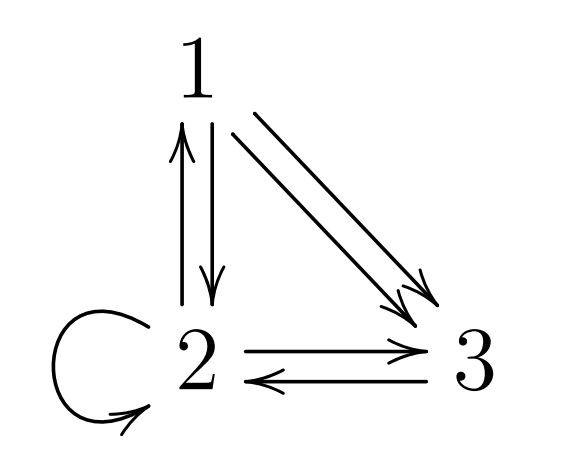
\includegraphics[scale=0.3]{188-HW5_Q3.png}\\ [-44pt]

Compute the rational function $P_{A;1,3}(x)$.

\begin{myIndent}\exOne
   Note that $A = \left[
   \begin{matrix}
      0 & 1 & 2 \\ 1 & 1 & 1 \\ 0 & 1 & 0
   \end{matrix}\right]$.\retTwo

   So: 
   \begin{center}
      \begin{tabular}{l}
         $P_{A;1,3}(x) = (-1)^{1 + 3}\frac{\det((\myId - xA); 3, 1)}{\det(\myId - xA)}$\\ [14pt]
         
         $\phantom{P_{A;1,3}(x)} = \frac{\det(\left[
         \begin{smallmatrix}
             -x & -2x \\ 1-x & -x
         \end{smallmatrix}\right])}{\det(\left[\begin{smallmatrix}
            1 & -x & -2x \\ -x & 1-x & -x \\ 0 & -x & 1
        \end{smallmatrix}\right])} = \frac{x^2 +2x - 2x^2}{1(1-x -x^2) + x(-x) -2x(x^2)} = \frac{x - x^2}{1 - x -2x^2 + 2x^3}$
      \end{tabular}
   \end{center}
   \retTwo\retTwo
\end{myIndent}

\blab{(4)} Construct a directed graph for which walks between certain vertices can be\\ interpreted as binary strings in which no symbol ever appears $3$ times in a row.

\begin{myIndent}\exOne
   Let $V = \{\text{binary strings of length } 2\} = \{00, 10, 01, 11\}$. Then given the words\\ $v = a_1a_2, u = b_1b_2 \in V$, we say there is an edge from $v$ to $u$ if $a_2 = b_1$ and\\ $a_1, a_2, b_1, b_2$ are not all equal. In other words, $(v, w)$ is an edge if $v$ and $w$ are\\ overlapping substrings of a word fulfilling our requirements.\retTwo

   This graph will look like: \phantom{aaaaaa}
   % https://q.uiver.app/#q=WzAsNCxbMCwwLCIwMCJdLFsxLDAsIjEwIl0sWzAsMSwiMDEiXSxbMSwxLCIxMSJdLFswLDJdLFsyLDNdLFszLDFdLFsxLDBdLFsxLDIsIiIsMSx7Im9mZnNldCI6MX1dLFsyLDEsIiIsMSx7Im9mZnNldCI6MX1dXQ==
   \begin{tikzcd}
   	00 & 10 \\
   	01 & 11
   	\arrow[from=1-1, to=2-1]
   	\arrow[from=2-1, to=2-2]
   	\arrow[from=2-2, to=1-2]
   	\arrow[from=1-2, to=1-1]
   	\arrow[shift right, from=1-2, to=2-1]
   	\arrow[shift right, from=2-1, to=1-2]
   \end{tikzcd}\retTwo

   There is a bijective correspondance between walks of length $k$ in the above graph and words of length $k + 2$. Specifically suppose $a_1 \cdots a_{k} a_{k+1} a_{k+2}$ is a binary word of length $k + 2$ where no symbol appears $3$ times in a rows. For $0 \leq i \leq k$, define $v_i = a_{i+1}a_{i+2}$. Then $v_0, v_1, \cdots, v_k$ is a walk of length $k$ in our graph.\retTwo

   To invert this process, if $v_0 = a_0b_0, v_1 = a_1b_1, \ldots, v_k = a_kb_k$ and $v_0, v_1, \ldots, v_n$ is a walk in our graph, then the word $a_0 b_0 b_1 \cdots b_k$ will be a binary word of length $k + 2$ with no symbol appearing $3$ times in a row.\newpage
\end{myIndent}

\blab{(5)} Let $A$ be a finite alphabet. We say that $\bm{w} = w_1\cdots w_k$ is a subword of\\ $\bm{v} = v_1\cdots v_n$ if there exists indices $1 \leq i_1 < i_2 < \cdots < i_k \leq n$ such that $v_{i_j} = w_j$ for all $j = 1, \ldots, n$. Define $a_{\bm{w}}(n)$ to be the number of words of length $n$ that have $\bm{w}$ as a subword. Prove that $\sum\limits_{n \geq 0}a_{\bm{w}}(n)x^n$ is a rational function of $x$.

\begin{myIndent}\exOne
   We shall proceed by induction on the length of $\bm{w}$.\retTwo

   To start, assume $\bm{w} = w_1$ is just a single symbol. Then there are $|A|^n$ many word of length $n$ and $(|A| - 1)^n$ of those don't have $\bm{w}$ as a substring (meaning that they don't contain the symbol $w_1$ and so are words of the alphabet $A - \{w_1\}$). So:\\ [-9pt]

   {\center 
   \begin{tabular}{l}
      $\sum\limits_{n \geq 0}a_{\bm{w}}(n)x^n = \sum\limits_{n \geq 0}(|A|x)^n - \sum\limits_{n \geq 0}((|A| - 1)x)^n$\\ [12pt]
      $\phantom{\sum\limits_{n \geq 0}a_{\bm{w}}(n)x^n} = \frac{1}{1 - |A|x} + \frac{1}{1 - |A|x + x} = \frac{2 - 2|A|x + x}{(1 - |A|x)(1 - |A|x + x)} = \frac{2 + (1 - 2|A|)x}{1 + (1 - 2|A|)x+ (|A|^2 - |A|)x^2}$
   \end{tabular} \retTwo\par}

   Now assume that $\sum\limits_{n \geq 0}a_{\bm{w}^\prime}(n)x^n$ is a rational function of $x$ for all words $\bm{w}^\prime$ of length\\ [-8pt] less than $k$.\retTwo

   Note that we can split the words $\bm{v}$ of length $n > 1$ with $\bm{w}$ as a subword into two types.
   \begin{itemize}
      \item Type 1: Suppose $w_1$ is not the first character of $\bm{v}$.
      
      \begin{myIndent}
         Then we must have that $\bm{w}$ is a substring of $v_2\cdots v_n$. Also, $v_1$ can be\\ any symbol in $A - \{w_1\}$. Concatting these substrings since they can be\\ chosen independently, there are $(|A| - 1)a_{\bm{w}}(n - 1)$ many words of this type.
      \end{myIndent}

      \item Type 2: Suppose $w_1 = v_1$.
      \begin{myIndent}
         Let $\bm{w}^\prime = w_2\cdots w_k$. Then we know that $\bm{w}^\prime$ is a substring $v_2 \cdots v_n$. So, the number of words of this type is $a_{\bm{w}^\prime}(n - 1)$.\retTwo
      \end{myIndent}
   \end{itemize}

   Clearly, if $n < 2 \leq k$, then $a_{\bm{w}}(n) = 0$. Also $a_{\bm{w}^\prime}(0) = 0$. So:\\ [-8pt]
   
   {\center
   \begin{tabular}{l}
      $\sum\limits_{n \geq 0}a_{\bm{w}}(n)x^n = \sum\limits_{n \geq 2}a_{\bm{w}}(n)x^n = \sum\limits_{n \geq 2}(|A| - 1)a_{\bm{w}}(n - 1)x^n + \sum\limits_{n \geq 2}a_{\bm{w}^\prime}(n-1)x^n$\\ [18pt]

      $\phantom{\sum\limits_{n \geq 0}a_{\bm{w}}(n)x^n = \sum\limits_{n \geq 2}a_{\bm{w}}(n)x^n} = (|A| - 1)x\sum\limits_{n \geq 1}a_{\bm{w}}(n)x^n + x\sum\limits_{n \geq 1}a_{\bm{w}^\prime}(n)x^n$\\ [18pt]

      $\phantom{\sum\limits_{n \geq 0}a_{\bm{w}}(n)x^n = \sum\limits_{n \geq 2}a_{\bm{w}}(n)x^n} = (|A| - 1)x\sum\limits_{n \geq 0}a_{\bm{w}}(n)x^n + x\sum\limits_{n \geq 0}a_{\bm{w}^\prime}(n)x^n$
   \end{tabular}\retTwo\par}

   By induction, we know that there are polynomials $P(x)$ and $Q(x)$ such that:
   
   {\centering $\sum\limits_{n \geq 0}a_{\bm{w}^\prime}(n)x^n = \frac{P(x)}{Q(x)}$.\retTwo\par}

   So, $(1 - (|A| - 1)x)\sum\limits_{n \geq 0}a_{\bm{w}}(n)x^n = \frac{xP(x)}{Q(x)}$.\newpage
   
   Hence, $\sum\limits_{n \geq 0}a_{\bm{w}}(n)x^n$ is the rational function $\frac{xP(x)}{(1 - (|A| - 1)x)Q(x)}$.\retTwo
   
   Now while that was all I was required to do, for the sake of fun I'm gonna also find an explicit formula for $\sum\limits_{n \geq 0}a_{\bm{w}}(n)x^n$.\retTwo

   Define $\bm{w}^{(i)} = w_i \cdots w_k$.\retTwo

   From before, we know that whenever $\bm{w}$ has length greater than $2$, we have that:
   
   {\centering $\sum\limits_{n \geq 0}a_{\bm{w}}(n)x^n = \frac{x}{1 - (|A| - 1)x} \cdot \sum\limits_{n \geq 0}a_{\bm{w}^\prime}(n)x^n$ \retTwo\par}

   So:\\ [-10pt]

   {\centering  
   \begin{tabular}{l}
      $\sum\limits_{n \geq 0}a_{\bm{w}}(n)x^n = \frac{x}{1 - (|A| - 1)x} \cdot \sum\limits_{n \geq 0}a_{\bm{w}^{(2)}}(n)x^n$\\ [18pt]
      
      $\phantom{\sum\limits_{n \geq 0}a_{\bm{w}}(n)x^n} = \left(\frac{x}{1 - (|A| - 1)x}\right)^2 \cdot \sum\limits_{n \geq 0}a_{\bm{w}^{(3)}}(n)x^n = \cdots = \left(\frac{x}{1 - (|A| - 1)x}\right)^{k-1} \sum\limits_{n \geq 0}a_{\bm{w}^{(k)}}(n)x^n$
   \end{tabular}\retTwo\par}

   Since $\bm{w}^{(n)}$ is a word of length 1, we know that $\sum\limits_{n \geq 0}a_{\bm{w}^{(n)}}(n)x^n = \frac{2 + (1 - 2|A|)x}{1 + (1 - 2|A|)x+ (|A|^2 - |A|)x^2}$.\retTwo

   So $\sum\limits_{n \geq 0}a_{\bm{w}}(n)x^n = \frac{x^{k-1}}{(1 - (|A| - 1)x)^{k-1}} \cdot \frac{2 + (1 - 2|A|)x}{1 + (1 - 2|A|)x+ (|A|^2 - |A|)x^2}$.\retTwo

   We can simplify this further. Note that:
   
   {\centering $(1 - 2|A|)^2 - 4(|A|^2 - |A|) = 1 - 4|A| + 4|A|^2 - 4|A|^2 + 4|A| = 1$.\retTwo\par}

   So by quadratic formula there is a scalar $c$ such that:
   
   {\centering 
   \begin{tabular}{l}
      $1 + (1 - 2|A|)x+ (|A|^2 - |A|)x^2 = c(x - \frac{2|A| - 2}{2|A|^2 - 2|A|})(x - \frac{2|A|}{2|A|^2 - 2|A|})$\\ [8pt]
      $\phantom{1 + (1 - 2|A|)x+ (|A|^2 - |A|)x^2} = c(x - \frac{1}{|A|})(x - \frac{1}{|A| - 1})$
   \end{tabular}\retTwo\par}

   By matching the $x^2$ terms, we know that $c = (|A|^2 - |A|)$. Thus, rearranging terms we get that:

   {\centering 
   \begin{tabular}{l}
      $1 + (1 - 2|A|)x+ (|A|^2 - |A|)x^2 = (|A|x - 1)((|A| - 1)x - 1)$\\
      $\phantom{1 + (1 - 2|A|)x+ (|A|^2 - |A|)x^2} = (1 - |A|x)(1 - (|A| - 1)x)$.
   \end{tabular} \retTwo\par}

   Therefore $\sum\limits_{n \geq 0}a_{\bm{w}}(n)x^n = \frac{2x^{k-1} + (1 - 2|A|)x^k}{(1 - (|A| - 1)x)^k(1 - |A|x)}$.\retTwo

   By our theorem on rational generating functions, we know there are constants\\ $c_1, \ldots, c_{k+1}$ such that if $N + k + 1 > k$, then for all $n \geq N$ we have that:

   {\centering $a_{\bm{w}}(n) = (c_1 + c_2n + \ldots + c_k n^{k-1})(|A| - 1)^n + c_{k+1}|A|^n$ \retTwo\par}

   $N = 0$ works for this. So for all $n \geq 0$ we have that:
   
   {\centering $a_{\bm{w}}(n) = (c_1 + c_2n + \ldots + c_k n^{k-1})(|A| - 1)^n + c_{k+1}|A|^n$\retTwo\par}
   
   To solve for each constant, use the initial conditions $a_{\bm{w}}(n) = 0$ when $n < k$ and $a_{\bm{w}}(k) = 1$. Unfortunately, I've run out of ideas for simplifying this more and it's 11:49PM.


   % {\centering 
   % \begin{tabular}{l}
   %    $\sum\limits_{n \geq 0}a_{\bm{w}}(n)x^n = (2x^{k-1} + (1 - 2|A|)x^k)\frac{1}{(1 - (|A| - 1)x)^k(1 - |A|x)}$\\
      
   %    $\phantom{\sum\limits_{n \geq 0}a_{\bm{w}}(n)x^n} = (x^k + 2x^{k-1}(1 - |A|x)) \frac{1}{(1 - (|A| - 1)x)^k(1 - |A|x)}$\\ 
      
   %    $\phantom{\sum\limits_{n \geq 0}a_{\bm{w}}(n)x^n} = \frac{x^k}{(1 - (|A| - 1)x)^k(1 - |A|x)} + \frac{2x^{k-1}}{(1 - (|A| - 1)x)^k}$\\

   %    $\phantom{\sum\limits_{n \geq 0}a_{\bm{w}}(n)x^n} = x^k(\sum\limits_{n \geq 0}\binom{k + n - 1}{n}(|A| - 1)^nx^n) + \frac{2x^{k-1}}{(1 - (|A| - 1)x)^k}$

   % \end{tabular}\retTwo\par}
\end{myIndent}

\end{document}

